

\documentclass[12pt]{book}

%%% preambulo
\input ../preambulo.tex
\input ../preambulo_counters.tex
\input ../preambulo_python.tex

\begin{document}

\frontmatter

% título
\title{Vetores}
\author{Pedro H A Konzen}
\date{\today}
\maketitle

% ficha catolográfica
\ifisbook
~
\vspace{4.5in}
\hrule
Konzen, Pedro Henrique de Almeida\\
\indent\hspace{2em}Vetores: notas de aula / Pedro Henrique de Almeida Konzen. --{\the\year}. Porto Alegre.- {\the\year}.\\
\indent\hspace{2em}"Esta obra é uma edição independente feita pelo próprio autor."\\
\indent\hspace{2em}1. Vetores. 2. Espaço euclidiano. 3. Base canônica.\\
\hrule
\vspace{1cm}
\begin{center}
  \textit{Licença}\\CC-BY-SA 4.0.
\end{center}
\fi

% licença
\chapter*{Licença}\label{licenca}
\addcontentsline{toc}{chapter}{Licença}

Este texto é disponibilizado sob a Licença Atribuição-CompartilhaIgual 4.0 Internacional Creative Commons. Para visualizar uma cópia desta licença, visite 
\begin{center}
  \url{http://creativecommons.org/licenses/by-sa/4.0/deed.pt\_BR} 
\end{center}
ou mande uma carta para Creative Commons, PO Box 1866, Mountain View, CA 94042, USA.


% prefácio


\chapter*{Prefácio}\label{prefacio}
\addcontentsline{toc}{chapter}{Prefácio}

O site \href{https://www.notaspedrok.com.br}{notaspedrok.com.br} é uma plataforma que construí para o compartilhamento de minhas notas de aula. Essas anotações feitas como preparação de aulas é uma prática comum de professoras/es. Muitas vezes feitas a rabiscos em rascunhos com validade tão curta quanto o momento em que são concebidas, outras vezes, com capricho de um diário guardado a sete chaves. Notas de aula também são feitas por estudantes - são anotações, fotos, prints, entre outras formas de registros de partes dessas mesmas aulas. Essa dispersão de material didático sempre me intrigou e foi o que me motivou a iniciar o site.

Com início em 2018, o site contava com apenas três notas incipientes. De lá para cá, conforme fui expandido e revisando os materais, o site foi ganhando acessos de vários locais do mundo, em especial, de países de língua portugusa. No momento, conta com 13 notas de aula, além de minicursos e uma coleção de vídeos e áudios.

As notas de \emph{Algoritmos e Programação I} fazem uma introdução a algoritmos e programação de computadores com a linguagem {\python}. É pensada para estudantes de cursos de matemática e áreas afins.

Aproveito para agradecer a todas/os que de modo assíduo ou esporádico contribuem com correções, sugestões e críticas. ;-)

\begin{flushright}
  Pedro H A Konzen\\\url{https://www.notaspedrok.com.br}
\end{flushright}



% toc
\ifishtml
\clearpage
\phantomsection
\addcontentsline{toc}{chapter}{Conteúdo}
\fi
\tableofcontents

\mainmatter

% 

\chapter{Introdução}\label{cap_intro}

Vamos começar executando nossas primeiras \emph{linhas de código} na linguagem de programação {\python}. Em um \emph{terminal} {\python} digitamos

\begin{lstlisting}
>>> print('Olá, mundo!')
\end{lstlisting}

Observamos que \lstinline+>>>+ é o símbolo do \lstinline+prompt de entrada+ e digitamos nossa \emph{instrução} logo após ele. Para executarmos a instrução digitada, teclamos \lstinline+<ENTER>+. Uma vez executada, o terminal apresentará as seguintes informações

\begin{lstlisting}
>>> print('Olá, mundo!')
Olá, mundo!
>>> 
\end{lstlisting}

Pronto! O fato do símbolo de \lstinline+prompt de entrada+ ter aparecido novamente, indica que a instrução foi completamente executada e o terminal está pronto para executar uma nova instrução.

A \emph{linha de comando} executada acima pede ao computador para imprimir no \lstinline+prompt de saída+ a frase \lstinline+Olá, mundo!+. O \emph{método} {\PYTHONprint} contém instruções para imprimir \emph{objetos} em um dispositivo de saída, no caso, imprime a frase na tela do computador.

Bem! Talvez imprimir no \lstinline+prompt de saída+ uma frase que digitamos no \lstinline+prompt de entrada+ possa parecer um pouco redundante no momento. Vamos considerar um outro exemplo, computar a soma dos números ímpares entre $0$ e $100$. Podemos fazer isso como segue

\begin{lstlisting}
>>> sum([i for i in range(100) if i%2 != 0])
2500
\end{lstlisting}

Oh! No momento, não se preocupe se não tenha entendido a linha de comando de entrada, ao longo dessas notas de aula isso vai ficando natural. A linha de comando de entrada usa o método {\PYTHONsum} para computar a soma dos elementos da \emph{lista} de números ímpares desejada. A lista é construída de forma \emph{iterada} e \emph{indexada} pela \emph{variável} \lstinline+i+, para \lstinline+i+ no intervalo/faixa de $0$ a $99$, se o resto da divisão de \lstinline+i+ por $2$ não for igual a $0$. Ok! O resultado computado foi $2500$.

De fato, a soma dos números ímpares de $0$ a $100$
\begin{equation}
  (1, 3, 5, \dotsc, 99)
\end{equation}
é a soma dos 50 primeiros elementos da progressão aritmética $a_i = 1 + 2i$, $i=0, 1, \ldots$, i.e.
\begin{align}
  \sum_{i=0}^{49}a_i &= a_0 + a_1 + \cdots + a_{49}\\
                     &= 1 + 3 + \cdots + 99\\
                     &= \frac{50(1 + 99)}{2}\\
                     &= 2500
\end{align}
como já esperado! Em {\python}, esta última conta pode ser computada como segue

\begin{lstlisting}
>>> 50*(1+99)/2
2500.0
\end{lstlisting}

%Este trabalho está licenciado sob a Licença Atribuição-CompartilhaIgual 4.0 Internacional Creative Commons. Para visualizar uma cópia desta licença, visite http://creativecommons.org/licenses/by-sa/4.0/deed.pt_BR ou mande uma carta para Creative Commons, PO Box 1866, Mountain View, CA 94042, USA.

\chapter{Fundamentos}\label{cap_vetor}

Neste capítulo, seguimos uma abordagem geométrica para introduzir os conceitos fundamentais e as operações básicas envolvendo vetores.

\section{Segmentos Orientados}\label{cap_vetor_sec_segorien}

O conceito de \hl{\emph{segmento orientado}} é fundamental na definição de vetores. Como o próprio nome indica, \hl{trata-se de definir uma orientação a um dado \emph{segmento de reta}}. Antes, portanto, vamos definir o que entendemos por um segmento.

\subsection{Segmento}
\badgeYouTube{J-GN-uulfRs}

\hl{Sejam dados dois pontos $A$ e $B$ sobre uma reta $r$. O conjunto de todos os pontos de $r$ entre $A$ e $B$ é chamado de \emph{segmento} e denotado por $AB$.} A reta $r$ é chamada de \emph{reta suporte} e os pontos $A$ e $B$ de \emph{pontos extremos}. Consulte a Figura~\ref{cap_vetor_sec_segorien:fig:segmento}.

\begin{figure}[h]
  \centering
  \includegraphics{./cap_vetor/dados/fig_segmento/fig.png}
  \caption{Um segmento $AB$ de uma reta (direção) $r$.}
  \label{cap_vetor_sec_segorien:fig:segmento}
\end{figure}

\subsubsection{Comprimento e Direção}

\hl{O \emph{comprimento} de um segmento $AB$ é denotado por $|AB|$ e definido como a distância entre seus pontos extremos $A$ e $B$}. Em outras palavras, é o tamanho do segmento\footnote{Em aplicações, o comprimento é medido em unidades de comprimento, metro $(m)$, no sistema internacional de unidades (SI).}. Consulte a Figura~\ref{cap_vetor_sec_segorien:fig:segmento_norma}

\begin{figure}[h]
  \centering
  \includegraphics{./cap_vetor/dados/fig_segmento_norma/fig.png}
  \caption{Comprimento de um segmento $AB$.}
  \label{cap_vetor_sec_segorien:fig:segmento_norma}
\end{figure}

\hl{A \emph{direção} de um segmento $AB$ é a direção de sua reta suporte}, i.e. a direção da reta que fica determinada pelos pontos $A$ e $B$. Logo, dois segmentos $AB$ e $CD$ têm a mesma direção, quando suas retas suportes são paralelas ou coincidentes (ou seja, elas têm a mesma direção).

\begin{figure}[h]
  \centering
  \includegraphics{./cap_vetor/dados/fig_segmento_direcao/fig.png}
  \caption{Segmentos de mesma direção $r\parallel s$.}
  \label{cap_vetor_sec_segorien:fig:segmento_direção.}
\end{figure}

\begin{ex}\label{cap_vetor_sec_segorien:ex:segmento}
  Consideramos os segmentos representados na Figura~\ref{cap_vetor_sec_segorien:fig:ex_segmento}. Observamos que $AB$ e $CD$ têm as mesmas direções, mas comprimentos diferentes. Já, o segmento $EF$ tem o mesmo comprimento que $AB$ (verifique!), mas tem direção diferente dos segmentos $AB$ e $CD$.
  
  \begin{figure}[h]
    \centering
    \includegraphics{./cap_vetor/dados/fig_ex_segmento/fig.png}
  \caption{Segmentos de diferentes comprimentos e direções.}
  \label{cap_vetor_sec_segorien:fig:ex_segmento}
\end{figure}
\end{ex}

\subsubsection{Segmento Nulo}

\hl{Se $A$ e $B$ são pontos coincidentes, então chamamos $AB$ de \emph{segmento nulo} e temos $|AB| = 0$.} Observamos que a representação geométrica de um segmento nulo é um ponto, tendo em vista que seus pontos extremos são coincidentes. Como existem infinitas retas de diferentes direções que passam por um único ponto, temos que \hl{segmentos nulos não têm direção definida}.

\subsection{Segmento Orientado}
\badgeYouTube{Mv0fW3\_6kVg}

Observamos que um dado segmento $AB$ é igual ao segmento $BA$. Agora, podemos associar a noção de \emph{sentido} a um segmento, escolhendo um dos pontos como sua \emph{origem} (ou \emph{ponto de partida}) e o outro como sua \emph{extremidade} (ou \emph{ponto de chegada}). Ao fazermos isso, definimos um \emph{segmento orientado}.

Mais precisamente, \hl{um segmento orientado $\overrightarrow{AB}$ é o segmento definido pelos pontos $A$ e $B$, sendo $A$ o ponto de partida (origem) e $B$ o ponto de chegada (extremidade)}. Consulte a Figura \ref{cap_vetor_sec_segorien:fig:seg_orientado}.

\begin{figure}[h]
  \centering
  \includegraphics{./cap_vetor/dados/fig_seg_orientado/fig.png}
  \caption{Um segmento orientado $\protect\overrightarrow{AB}$.}
  \label{cap_vetor_sec_segorien:fig:seg_orientado}
\end{figure}

\subsubsection{Comprimento e Direção}

As noções de comprimento e de direção para segmentos estendem-se diretamente a segmentos orientados. Dizemos que dois \hl{segmentos orientados não nulos $\overrightarrow{AB}$ e $\overrightarrow{CD}$ têm a \textbf{mesma direção}, quando as retas $AB$ e $CD$ são paralelas ou coincidentes}. Em outras palavras, dois segmentos orientados não nulos têm a mesma direção quando suas retas suporte são paralelas ou coincidentes.

  \hl{O \emph{comprimento} de um segmento orientado $\overrightarrow{AB}$ é a norma do segmento $AB$}, i.e. $\left|\overrightarrow{AB}\right| = |AB|$. O segmento orientado nulo $\overrightarrow{AA}$ tem comprimento $\left|\overrightarrow{AA}\right|=0$ e não tem direção definida.

\subsubsection{Sentido}
\badgeYouTube{nT0VUIp7nIM}

\hl{O \emph{sentido} de um segmento orientado é o do ponto de partida (origem) para o ponto de chegada (extremo)}. Por exemplo, o segmento orientado $\overrightarrow{AB}$ tem sentido do ponto $A$ ao $B$.

\hl{Segmentos orientados $\overrightarrow{AB}$ e $\overrightarrow{CD}$ de mesma direção} podem ter o mesmo sentido ou sentidos opostos. No caso de suas retas suportes não serem coincidentes, os segmentos orientados $\overrightarrow{AB}$ e $\overrightarrow{CD}$ \hl{têm o mesmo sentido, quando os segmentos $AC$ e $BD$ não se interceptam. No contrário, caso estes se interceptam, os segmentos orientados $\overrightarrow{AB}$ e $\overrightarrow{CD}$ têm sentidos opostos}. 

\begin{ex}
  Na Figura~\ref{cap_vetor_sec_segorien:fig:segorien_sentido}, temos que os segmentos $\overrightarrow{AB}$ e $\overrightarrow{CD}$ têm o mesmo sentido. De fato, observamos que eles têm a mesma direção e que os segmentos $AC$ e $BD$ têm interseção vazia.

\begin{figure}[h]
  \centering
  \includegraphics{./cap_vetor/dados/fig_segorien_sentido/fig.png}
  \caption{Segmentos orientados $\protect\overrightarrow{AB}$ e $\protect\overrightarrow{CD}$ de mesmo sentido. Segmentos orientados $\protect\overrightarrow{EF}$ e $\protect\overrightarrow{GH}$ de sentidos opostos.}
  \label{cap_vetor_sec_segorien:fig:segorien_sentido}
\end{figure}

Na mesma Figura~\ref{cap_vetor_sec_segorien:fig:segorien_sentido}, temos que os segmentos orientados $\overrightarrow{EF}$ e $\overrightarrow{GH}$ têm sentidos opostos, pois têm a mesma direção e os segmentos $EG$ e $FH$ se interceptam. 
\end{ex}

\begin{obs}\normalfont{(\hl{Transitividade do sentido}.)}\label{cap_vetor_sec_segorien:obs:segorin_sentido_trans}
  \hl{A propriedade de segmentos orientados terem o mesmo sentido é transitiva}. Ou seja, se $\overrightarrow{AB}$ e $\overrightarrow{CD}$ têm o mesmo sentido e $\overrightarrow{CD}$ e $\overrightarrow{EF}$ têm o mesmo sentido, então $\overrightarrow{AB}$ e $\overrightarrow{EF}$ têm o mesmo sentido.
\end{obs}

Com base na Observação~\ref{cap_vetor_sec_segorien:obs:segorin_sentido_trans}, analisamos o sentido de dois segmentos orientados e colineares escolhendo um deles e construindo um segmento orientado de mesmo sentido e não colinear. Então, analisamos o sentido dos segmentos orientados originais com respeito ao introduzido.

\subsubsection{Relação de Equipolência}
\badgeYouTube{CgfyqqvhBng}

\hl{Um segmento orientado não nulo $\overrightarrow{AB}$ é \emph{equipolente} a um segmento orientado $\overrightarrow{CD}$, quando $\overrightarrow{AB}$ tem o \emph{mesmo comprimento}, a \emph{mesma direção} e o \emph{mesmo sentido} de $\overrightarrow{CD}$} (consulte a Figura~\ref{cap_vetor_sec_segorien:fig:segequipolentes}). Segmentos nulos também são considerados equipolentes entre si. 

Usamos a notação \hl{$\overrightarrow{AB} \sim \overrightarrow{CD}$} para indicar que $\overrightarrow{AB}$ é equipolente a $\overrightarrow{CD}$. Caso contrário, escrevemos \hl{$\overrightarrow{AB} \not\sim \overrightarrow{CD}$}.

\begin{figure}[h]
  \centering
  \includegraphics{./cap_vetor/dados/fig_segequipolentes/fig.png}
  \caption{Dois segmentos orientados equipolentes.}
  \label{cap_vetor_sec_segorien:fig:segequipolentes}
\end{figure}

\hl{A relação de equipolência é uma \emph{relação de equivalência}}. De fato, temos:
\begin{itemize}
\item \emph{relação reflexiva}: $\overrightarrow{AB} \sim \overrightarrow{AB}$;
\item \emph{relação simétrica}: $\overrightarrow{AB} \sim \overrightarrow{CD} \Rightarrow \overrightarrow{CD} \sim \overrightarrow{AB}$;
\item \emph{relação transitiva}: $\overrightarrow{AB} \sim \overrightarrow{CD} ~ \text{e} ~ \overrightarrow{CD} \sim \overrightarrow{EF} \Rightarrow \overrightarrow{AB} \sim \overrightarrow{EF}$.
\end{itemize}

Com isso, \hl{dado um segmento orientado $\overrightarrow{AB}$, definimos a \emph{classe de equipolência} de $\overrightarrow{AB}$ como o conjunto de todos os seus segmentos equipolentes}. O segmento $\overrightarrow{AB}$ é um \emph{representante} desta classe, a qual é denotada por $\left[\overrightarrow{AB}\right]_{\sim}$.

\subsection{Exercícios Resolvidos}

\begin{exeresol}
  Sejam dados três pontos não colineares $A$, $B$ e $D$. Escreva a área do paralelogramo determinado pelos segmentos $AB$ e $AD$ com respeito aos comprimentos deles e ao ângulo determinado por eles.
\end{exeresol}
\begin{resol}
  Começamos desenhando um paralelogramo determinado por segmentos $AB$ e $AD$. Consulte a Figura~\ref{cap_vetor_sec_segorien:fig:exeresol_paralelogramo}.

  \begin{figure}[H]
    \centering
    \includegraphics{./cap_vetor/dados/fig_exeresol_paralelogramo/fig.png}
    \caption{Paralelogramo determinado por segmentos $AB$ e $AD$.}
    \label{cap_vetor_sec_segorien:fig:exeresol_paralelogramo}
  \end{figure}

  Denotando por $\alpha$ o ângulo determinado pelos segmentos $AB$ e $AD$, temos que a área deste paralelogramo pode ser escrita por
  \begin{equation}
    A = |AB|\cdot |AD| \sen \alpha.
  \end{equation}
\end{resol}

\begin{exeresol}
  Mostre que $\overrightarrow{AB}\sim \overrightarrow{CD}$ se, e somente se, $\overrightarrow{BA}\sim \overrightarrow{DC}$.
\end{exeresol}
\begin{resol}
  Para mostrar que
  \begin{equation}
    \overrightarrow{AB}\sim \overrightarrow{CD} \Leftrightarrow \overrightarrow{BA}\sim \overrightarrow{DC},
  \end{equation}
  vamos primeiro mostrar a implicação, i.e. que
  \begin{equation}
    \overrightarrow{AB}\sim \overrightarrow{CD} \Rightarrow \overrightarrow{BA}\sim \overrightarrow{DC}.
  \end{equation}
  Logo, assumimos que $\overrightarrow{AB}\sim \overrightarrow{CD}$, mostramos que
  \begin{enumerate}[a)]
    \item $\left|\overrightarrow{BA}\right| = \left|\overrightarrow{DC}\right|$.
    
      De fato, temos
      \begin{equation}
        \left|\overrightarrow{BA}\right| = \left|\overrightarrow{AB}\right| \overset{\sim}{=} \left|\overrightarrow{CD}\right| = \left|\overrightarrow{DC}\right|.
      \end{equation}

    \item $\overrightarrow{BA}$ e $\overrightarrow{DC}$ têm as mesmas direções.
    
      A direção de $\overrightarrow{BA}$ é a mesma de $\overrightarrow{AB}$, pois suas retas suportes são coincidentes. Pela equipolência, essa também é a direção de $\overrightarrow{CD}$. Por fim,  $\overrightarrow{CD}$ e $\overrightarrow{DC}$ têm a mesma direção, pois suas retas suportes são coincidentes. O resultado segue por transitividade.
      
    \item $\overrightarrow{BA}$ e $\overrightarrow{DC}$ têm os mesmos sentidos.
    
      Como, por hipótese, $\overrightarrow{AB}$ tem o mesmo sentido de $\overrightarrow{CD}$, temos que os segmentos $AC$ e $BD$ não se interceptam. Isto, por sua vez, mostra que $\overrightarrow{BA}$ e $\overrightarrow{DC}$ têm o mesmo sentido.
  \end{enumerate}

  Dos items, a), b) e c), concluímos que
  \begin{equation}
    \overrightarrow{AB}\sim \overrightarrow{CD} \Rightarrow \overrightarrow{BA}\sim \overrightarrow{DC}.
  \end{equation}

  Para mostrar a recíproca, i.e. que
  \begin{equation}
    \overrightarrow{AB}\sim \overrightarrow{CD} \Leftarrow \overrightarrow{BA}\sim \overrightarrow{DC}.
  \end{equation}
  basta substituir $\overrightarrow{AB}$ ($\overrightarrow{BA}$) por $\overrightarrow{BA}$ ($\overrightarrow{AB}$) e $\overrightarrow{CD}$ ($\overrightarrow{DC}$) por $\overrightarrow{DC}$ ($\overrightarrow{CD}$) nos itens a), b) e c) demonstrados acima. Em outras palavras, a demonstração é anaĺoga. Verifique!
\end{resol}

\subsection{Exercícios}

\begin{exer}
  Complete as lacunas.
  \begin{enumerate}[a)]
    \item Seja $r$ a reta determinada pelos pontos $A$ e $B$. O segmento $AB$ é o conjunto de \underline{\phantom{pontos}} pertencentes a $r$ e que estão \underline{\phantom{entre}} $A$ e $B$ (inclusive). 
    \item O comprimento de um segmento $AB$ é definido como a \underline{\phantom{distância}} entre $A$ e $B$ e é denotada por \underline{\phantom{|AB|}}.
    \item Chamamos de \underline{\phantom{reta suporte}} de um dado segmento $AB$, a reta determinada pelos pontos $A$ e $B$.
    \item $AB$ é dito ser um segmento nulo, quando $A$ e $B$ são pontos \underline{\phantom{coincidentes}}.
  \end{enumerate}
\end{exer}
\begin{resp}
  a) pontos; entre; c) distância; $|AB|$; d) reta suporte; e) coincidentes;
\end{resp}

\begin{exer}
  Complete as lacunas.
  \begin{enumerate}[a)]
    \item Segmento orientado é um segmento com \underline{\phantom{sentido}} definido.
    \item Em um segmento orientado $\overrightarrow{AB}$, $A$ é chamado de \underline{\phantom{ponto de origem}} e \underline{\phantom{ponto de extremidade}}.
    \item Se as retas $AB$ e $CD$ são paralelas ou coincidentes, então $\overrightarrow{AB}$ e $\overrightarrow{CD}$ têm a mesma \underline{\phantom{direção}}.
    \item O comprimento de um segmento orientado $\overrightarrow{AB}$ é definido como o comprimento do segmento \underline{\phantom{|AB|}}.
    \item $\overrightarrow{AB}$ e $\overrightarrow{CD}$ têm \underline{\phantom{o mesmo sentido (sentidos opostos)}} quando os segmentos $AC$ e $BD$ não se interceptam (se interceptam).
  \end{enumerate}
\end{exer}
\begin{resp}
  a) sentido; b) ponto de origem; ponto de extremidade;  c) direção; d) $|AB|$; e) o mesmo sentido (sentidos opostos); não se interceptam (se interceptam)
\end{resp}

\begin{exer}
  Complete as lacunas.
  \begin{enumerate}[a)]
    \item $\overrightarrow{AB}$ e $\overrightarrow{CD}$ são \underline{\phantom{equipolentes}} se, e somente se, $\overrightarrow{AB}$ e $\overrightarrow{CD}$ têm a mesma \underline{\phantom{direção}}, o mesmo \underline{\phantom{comprimento}} e o mesmo \underline{\phantom{sentido}}.
    \item Pela reflexividade da relação de equipolência, $\overrightarrow{CD}\sim$ \underline{\phantom{$\overrightarrow{CD}$}}.
    \item Pela simetria da relação de equipolência, se $\overrightarrow{EF}\sim\overrightarrow{AB}$, então \underline{\phantom{$\overrightarrow{AB}\sim\overrightarrow{EF}$}}.
    \item Pela transitividade da relação de equipolência, se $\overrightarrow{CD}\sim\overrightarrow{AB}$ e \underline{\phantom{$\overrightarrow{AB}\sim\overrightarrow{EF}$}}, então $\overrightarrow{CD}\sim\overrightarrow{EF}$.
  \end{enumerate}
\end{exer}
\begin{resp}
  a) equipolentes; direção; comprimento; sentido; b) $\overrightarrow{CD}$; c) $\overrightarrow{AB}\sim\overrightarrow{EF}$; d) $\overrightarrow{AB}\sim\overrightarrow{EF}$
\end{resp}

\begin{exer}\label{cap_vetor_sec_segorien:fig:exer_segs_dif_normas}
  Faça o esboço de dois segmentos $AB$ e $CD$ com $|AB|\neq |CD|$ e cujas retas determinadas por eles sejam coincidentes.
\end{exer}
\begin{resp}

  \includegraphics{./cap_vetor/dados/fig_exer_segs_dif_normas/fig.png}
\end{resp}

\begin{exer}\label{cap_vetor_sec_segorien:fig:exer_segs_nems}
  Faça o esboço de dois segmentos orientados $AB\not\sim CD$ e de mesmo sentido.
\end{exer}
\begin{resp}
  
  \includegraphics{./cap_vetor/dados/fig_exer_segs_nems/fig.png}
\end{resp}

\begin{exer}\label{cap_vetor_sec_segorien:fig:exer_segs_hn_s}
  Faça o esboço de dois segmentos orientados colineares, de comprimentos iguais e sentidos opostos.
\end{exer}
\begin{resp}
  
  \includegraphics{./cap_vetor/dados/fig_exer_segs_hn_s/fig.png}
\end{resp}

\begin{exer}
  Mostre que segmentos terem o mesmo comprimento é uma:
  \begin{enumerate}[a)]
    \item relação reflexiva.
    \item relação simétrica.
    \item relação transitiva.
    \item relação de equivalência.
  \end{enumerate}
\end{exer}
\begin{resp}
  a) Por óbvio, que $AB$ tem o mesmo comprimento que si próprio. b) Se $AB$ tem o mesmo comprimento de $CD$, $|AB| = |CD|$, então é dizer que $CD$ tem o mesmo comprimento de $AB$. c) Se $|AB| = |CD|$ e $|CD| = |EF|$, então $|AB| = |EF|$. d) Por definição, segue dos itens $a)$, $b)$ e $c)$.
\end{resp}

\begin{exer}
  Mostre que $\overrightarrow{AB}\sim \overrightarrow{CD}$, então $\overrightarrow{AC}\sim \overrightarrow{BD}$.
\end{exer}
\begin{resp}
  Dica: Se $\overrightarrow{AB}$ e $\overrightarrow{CD}$ não são coincidentes, então $ABCD$ determina um paralelogramo.
\end{resp}

\begin{exer}
  Mostre que se $AC\sim CB$, então $C$ é ponto médio do segmento $AB$.
\end{exer}
\begin{resp}
  $AC\sim CB$ implica que $C\in AB$. Como $\left|\overrightarrow{AC}\right| = \left|\overrightarrow{CB}\right|$, conclui-se que $C$ é o ponto médio de $AB$.
\end{resp}

\begin{exer}
  Mostre que se $\overrightarrow{AB}$ e $\overrightarrow{CD}$ são equipolentes, então os pontos médios de $AD$ e $BC$ são coincidentes.
\end{exer}
\begin{resp}
  Dica: as diagonais de um paralelogramo interceptam-se em seus pontos médios.
\end{resp}

\ifisbook
\subsubsection{Respostas}
\shipoutAnswer
\fi

\section{Definição de Vetor}\label{cap_vetor_sec_vetor}
\badgeYouTube{2qxgs37JNBo}

% \begin{flushright}
%   \href{https://archive.org/details/definicao-vetor}{$\blacktriangleright$ Vídeo disponível!}
% \end{flushright}

\hl{Um \emph{vetor} $\vec{u}$ é definido como a \emph{classe de equipolência}\footnote{Consulte a Seção~\ref{cap_vetor_sec_segorien} para a definição de classe de equipolência.} dos \emph{segmentos orientados} $\overrightarrow{AB}$ de dado \emph{comprimento}, dada \emph{direção} e dado \emph{sentido}}, i.e. $\vec{u} = \left[\overrightarrow{AB}\right]_{\sim}$. Qualquer $\overrightarrow{AB}\in \left[\overrightarrow{AB}\right]_{\sim}$ é uma \emph{representação do vetor} $\vec{u}$ como um segmento orientado. Consulte a Figura~\ref{cap_vetor_sec_vetor:fig:vetor}.

\begin{figure}[h]
  \centering
  \includegraphics{./cap_vetor/dados/fig_vetor/fig.png}
  \caption{Duas representações de dado vetor $\vec{u}$.}
  \label{cap_vetor_sec_vetor:fig:vetor}
\end{figure}

\begin{obs}\normalfont{(\hl{Notação}.)}
  Para simplificar a notação, usualmente, escrevemos $\vec{u}=\overrightarrow{AB}$ no lugar de $\vec{u} = \left[\overrightarrow{AB}\right]_{\sim}$.
\end{obs}

\hl{A \emph{norma} de um vetor $\vec{u}$ é denotada por $\|\vec{u}\|$ e definida como o comprimento de qualquer uma de suas representações}. Mais precisamente, se o segmento orientado $\overrightarrow{AB}$ é uma representação de $\vec{u}$, i.e. $\vec{u} = \overrightarrow{AB}$, então
\begin{equation}
  \|\vec{u}\| := |\overrightarrow{AB}| := |AB|.
\end{equation}
Consulte a Figura~\ref{cap_vetor_sec_vetor:fig:vetor_norma}.

\begin{figure}[h]
  \centering
  \includegraphics{./cap_vetor/dados/fig_vetor_norma/fig.png}
  \caption{Norma de um vetor $\vec{u}$.}
  \label{cap_vetor_sec_vetor:fig:vetor_norma}
\end{figure}

\hl{O \emph{vetor nulo} é aquele que tem como representante um segmento orientado nulo}. É denotado por $\vec{0}$ e geometricamente representado por um ponto.

\begin{proposicao}\normalfont{(\hl{Vetor Nulo}.)}
  $\|\vec{u}\| = 0$ se, e somente se, $\vec{u} = \vec{0}$.
\end{proposicao}
\begin{demonstracao}
  Primeiramente, vamos mostrar a implicação. Por hipótese, temos que $\|\vec{u}\| = 0$. Seja, $\overrightarrow{AB}$ uma representação de $\vec{u}$. Então, por definição da norma de vetor, $\|\vec{u}\| := \left|\overrightarrow{AB}\right| = 0$. Logo, $AB$ é um segmento nulo, i.e. $A$ é coincidente a $B$ e, portanto, $\vec{u} = \vec{0}$.

  Agora, mostramos a recíproca, i.e., se $\vec{u} = \vec{0}$, então $\|\vec{u}\| = 0$. Como $\vec{u} = \vec{0}$, temos que $\vec{u}$ pode ser representado por qualquer segmento orientado $\overrightarrow{AA}$. Temos que $\left|\overrightarrow{AA}\right| = 0$ e, portanto, $\|\vec{u}\| := \left|\overrightarrow{AA}\right| = 0$.
\end{demonstracao}

Usualmente, escolhemos um ponto $O$ como origem do espaço. A seguinte proposição, garante que \hl{todo o vetor admite uma única representação a partir dessa origem}.

\begin{proposicao}\normalfont{(\hl{Representação de Vetor a partir da Origem})}\label{cap_vetor_sec_vetor:prop:vetor_origem}
  Seja dado um ponto $O$ no espaço. Todo vetor $\vec{u}$ admite uma única representação $\overrightarrow{OA}$.
\end{proposicao}
\begin{demonstracao}
  Seja dado um ponto $O$ e um vetor $\vec{u}$. Começamos por \emph{mostrar a existência}, i.e. que existe $A$ tal que $\vec{u}=\overrightarrow{OA}$. Seja $\overrightarrow{BC}$ uma representação de $\vec{u}$ e $r$ sua reta suporte. Seja, então, $s$ a reta que passa pelo ponto $O$ e é paralela (ou coincidente) a $r$.  Consulte a Figura~\ref{cap_vetor_sec_vetor:fig:vetor_origem}.
  
  \begin{figure}[h!]
    \centering
    \includegraphics{./cap_vetor/dados/fig_vetor_origem/fig.png}
    \caption{Representação de um vetor a partir da origem do espaço.}
    \label{cap_vetor_sec_vetor:fig:vetor_origem}
  \end{figure}
  
  Escolhemos, então, $A\in p$ tal que $|OA| = \left|\overrightarrow{BC}\right|$ e tal que $\overrightarrow{OA}$ tenha o mesmo sentido de $\overrightarrow{BC}$. Logo, $\overrightarrow{BC}$ é equipolente a $\overrightarrow{OA}$, que é a representação desejada de $\vec{u}$.

  Agora, vamos \emph{mostrar a unicidade}, i.e. que se $A$ e $B$ são pontos tais que $\vec{u}=\overrightarrow{OA}\sim\overrightarrow{OB}$, então $A$ e $B$ são coincidentes. \emph{Por negação}, se $A$ e $B$ não forem coincidentes, então $O$, $A$ e $B$ são pontos colineares ou não, exclusivamente. Neste caso, $\overrightarrow{OA}$ e $\overrightarrow{OB}$ não tem a mesma direção. Noutro caso, $|\overrightarrow{OA}| \neq |\overrightarrow{OB}|$ ou $\overrightarrow{OA}$ e $\overrightarrow{OB}$ têm sentidos opostos. Em qualquer um dos casos $\overrightarrow{OA}\not\sim\overrightarrow{OB}$.
\end{demonstracao}

\hl{Dois vetores não nulos determinam um único ângulo}\footnote{Mais precisamente, uma classe de ângulos congruentes}.

\begin{proposicao}\normalfont{(\hl{Ângulo entre Vetores}.)}
  Dois vetores não nulos determinam uma única classe de ângulos congruentes.
\end{proposicao}
\begin{demonstracao}
  Existência. Sejam dados os vetores $\vec{u}$ e $\vec{v}$ não nulos e suas representações $\vec{u}=\overrightarrow{OA}$ e $\vec{v}=\overrightarrow{OB}$. Logo, $OA$ e $OB$ determinam duas semi-retas de ângulo $\hat{O}$ (consulte a Figura~\ref{cap_vetor_sec_vetor:fig:vetores_e_angulos}).

  \begin{figure}[h!]
    \centering
    \includegraphics{./cap_vetor/dados/fig_vetores_e_angulos/fig.png}
    \caption{Dois vetores determinam um ângulo.}
    \label{cap_vetor_sec_vetor:fig:vetores_e_angulos}
  \end{figure}

  Unicidade. Sejam dois ângulos $\hat{O}$ e $\hat{O}'$ determinados pelos vetores $\vec{u}$ e $\vec{v}$. Sejam, também, as representações $\vec{u}=\overrightarrow{OA}=\overrightarrow{O'A'}$ e $\vec{v}=\overrightarrow{OB}=\overrightarrow{O'B'}$. Logo, as semi-retas $OA$ e $O'A'$ têm as mesmas direções. Bem como, as semi-retas $OB$ e $O'B'$ têm as mesmas direções. Concluímos que os ângulos $\hat{O}$ e $\hat{O}'$ são congruentes.
\end{demonstracao}

\hl{Dois \textbf{vetores} são ditos \textbf{paralelos} quando admitem representações paralelas}. De forma análoga, definem-se \textbf{vetores coplanares}, \textbf{vetores não coplanares}, \textbf{vetores ortogonais}, etc.

\begin{ex}
  Na Figura~\ref{cap_vetor_sec_vetor:fig:vetores_pararel_perp}, temos $\vec{u}$ vetor paralelo a $\vec{v}$, enquanto que $\vec{x}$ é ortogonal a $\vec{y}$.

  \begin{figure}[h]
    \centering
    \includegraphics{./cap_vetor/dados/fig_vetores_paralelos/fig.png} ~
    \includegraphics{./cap_vetor/dados/fig_vetores_ortogonais/fig.png}
    \caption{Vetores paralelos $\vec{u}\parallel\vec{v}$ e vetores ortogonais $\vec{x}\perp\vec{y}$.}
    \label{cap_vetor_sec_vetor:fig:vetores_pararel_perp}
  \end{figure}

  Agora, na Figura~\ref{cap_vetor_sec_vetor:fig:vetores_coplanares}, temos que os vetores $\vec{a}$, $\vec{b}$ e $\vec{c}$ são coplanares.

  \begin{figure}[h]
    \centering
    \includegraphics[width=2.5in]{./cap_vetor/dados/fig_vetores_coplanares/fig.png}
    \caption{Vetores coplanares.}
    \label{cap_vetor_sec_vetor:fig:vetores_coplanares}
  \end{figure}
  
\end{ex}


\subsection{Exercícios Resolvidos}

\begin{exeresol}
  Mostre que um plano fica unicamente determinado por um ponto e dois vetores não nulos de diferentes direções.
\end{exeresol}
\begin{resol}
  Primeiramente, vamos mostrar a existência de um plano $\alpha$ tal que $O, \vec{u}, \vec{v}\in\alpha$ (consulte a Figura~\ref{cap_vetor_sec_vetor:fig:vetores_e_planos}). Sejam um ponto $O$ e dois vetores $\vec{u}$ e $\vec{v}$ não nulos e de diferentes direções. Escolhemos, então, suas representações $\vec{u} = \overrightarrow{OA}$ e $\vec{v} = \overrightarrow{OB}$. Como $\vec{u}$ e $\vec{v}$ não nulos e têm diferentes direções, temos que os pontos $O$, $A$ e $B$ são não colineares. Logo, estes pontos determinam um plano $\alpha$, tal que $O, \vec{u}, \vec{v} \in \alpha$.

  \begin{figure}[h!]
    \centering
    \includegraphics[width=4in]{./cap_vetor/dados/fig_vetores_e_planos/fig.png}
    \caption{Vetores e planos.}
    \label{cap_vetor_sec_vetor:fig:vetores_e_planos}
  \end{figure}
  
  A unicidade segue imediatamente do fato de que três pontos não colineares determinam unicamente um plano.

\end{resol}

\begin{exeresol}\label{cap_vetor_sec_vetor:exeresol:vetores_e_paralelogramos}
  Mostre que dois vetores não nulos e de diferentes direções determinam unicamente uma classe de paralelogramos congruentes\footnote{Dois polígonos são congruentes, quando seus lados e ângulos correspondentes têm a mesma medida.}.
\end{exeresol}
\begin{resol}
  Existência. Sejam $\vec{u}$ e $\vec{v}$ dois vetores não nulos e de diferentes direções. Sejam, então, suas representações $\vec{u}=\overrightarrow{AB}$ e $\vec{v}=\overrightarrow{AD}$ (consulte a Figura~\ref{cap_vetor_sec_vetor:fig:vetores_e_paralelogramos}). Sejam, agora, as retas $r$ e $s$ tais que $B\in r$, $r\parallel\vec{v}$, $D\in s$ e $s\parallel\vec{u}$. Seja, $C$ o ponto de interseção de $r$ e $s$. Por construção, temos que $AB\parallel DC$ e $AD\parallel BC$, o que mostra que $ABCD$ é um paralelogramo.

  \begin{figure}[h!]
    \centering
    \includegraphics{./cap_vetor/dados/fig_vetores_e_paralelogramos/fig.png}
    \caption{Paralelogramo determinado por vetores não nulos de diferentes direções.}
    \label{cap_vetor_sec_vetor:fig:vetores_e_paralelogramos}
  \end{figure}
  
  Unicidade. Falta mostrar que, dados $\vec{u}$ e $\vec{v}$ vetores não nulos e de diferentes direções, então são congruentes quaisquer dois paralelogramos determinados por $\vec{u}$ e $\vec{v}$. Consulte o exercício \exerref{cap_vetor_sec_vetor:exer:vetores_e_paralelogramos}.
  
\end{resol}

\subsection{Exercícios}

\begin{exer}
  Complete as lacunas.
  \begin{enumerate}[a)]
    \item Um vetor é definido por sua \underline{\phantom{norma}}, direção e \underline{\phantom{sentido}}.
    \item Se $\vec{u}$ tem representação $\overrightarrow{AB}$, então $\|\vec{u}\|=$\underline{\phantom{$\left|\overrightarrow{AB}\right|$}}.
    \item Se $\|\vec{v}\|=0$, então $\vec{v}$ é um \underline{\phantom{vetor nulo}}.
    \item Vetores paralelos são vetores de mesma/o \underline{\phantom{direção}}.
  \end{enumerate}
\end{exer}
\begin{resp}
  a) norma; sentido. b) $\left|\overrightarrow{AB}\right|$. c) vetor nulo. d) direção.
\end{resp}

\begin{exer}
  Diga se é verdadeira ou falsa cada uma das seguintes afirmações:
  \begin{enumerate}[a)]
    \item Todos os vetores podem ser representados a partir de um mesmo ponto de origem.
    \item Dois vetores de mesma norma são vetores paralelos.
    \item Dois vetores são sempre coplanares entre si.
  \end{enumerate}
\end{exer}
\begin{resp}
  a) V. b) F. c) V.
\end{resp}

\begin{exer}
  Diga se é verdadeira ou falsa cada uma das seguintes afirmações:
  \begin{enumerate}[a)]
    \item Dois vetores não nulos determinam uma única classe de ângulos congruentes.
    \item Dois vetores não nulos de diferentes direções determinam um único plano.
    \item Dois vetores não nulos de diferentes direções determinam uma única classe de paralelogramos congruentes.
  \end{enumerate}
\end{exer}
\begin{resp}
  a) V. b) F. c) V.
\end{resp}

\begin{exer}
  Com base na figura abaixo, qual(is) dos vetores indicados são iguais ao vetor $\overrightarrow{AB}$.
  \begin{figure}[H]
    \centering
    \includegraphics[width=0.7\textwidth]{./cap_vetor/dados/fig_exer_definicao_01/fig_exer_definicao_01}
  \end{figure}
\end{exer}
\begin{resp}
  $\vec{w}, \vec{c}$
\end{resp}

\begin{exer}
  Sejam $A$, $B$ e $C$ pontos dois a dois distintos. Se $\vec{b}$ é um vetor nulo, então $\vec{b}$ é igual a:
  \begin{enumerate}[a)]
  \item $\vec{0}$
  \item $\overrightarrow{AB}$
  \item $\overrightarrow{CC}$
  \item $\overrightarrow{CA}$
  \item $\overrightarrow{BB}$
  \end{enumerate}
\end{exer}
\begin{resp}
  a), c), e) 
\end{resp}

\begin{exer}
  Com base na figura abaixo, qual(is) dos vetores indicados são paralelos entre si.
  \begin{figure}[H]
    \centering
    \includegraphics[width=0.7\textwidth]{./cap_vetor/dados/fig_exer_definicao_01/fig_exer_definicao_01}
  \end{figure}
\end{exer}
\begin{resp}
  $\vec{d}\parallel\vec{e}$; $\vec{c}\parallel\vec{v}\parallel\vec{w}$
\end{resp}

\begin{exer}
  Com base na figura abaixo, qual(is) dos vetores indicados são ortogonais (perpendiculares) entre si.
  \begin{figure}[H]
    \centering
    \includegraphics[width=0.7\textwidth]{./cap_vetor/dados/fig_exer_definicao_01/fig_exer_definicao_01}
  \end{figure}
\end{exer}
\begin{resp}
  $\vec{e}\perp\vec{m}$.
\end{resp}

\begin{exer}
  Mostre que uma reta fica unicamente determinada por um ponto $O$ e um vetor não nulo $\vec{u}$.
\end{exer}
\begin{resp}
  Seja $A$ tal que $\vec{u} = \overrightarrow{OA}$. Como $\vec{u}\neq\vec{0}$, temos que $O$ e $A$ são não coincidentes. Temos então, uma única reta $r$ tal que $O,A\in r$.
\end{resp}

\begin{exer}\label{cap_vetor_sec_vetor:exer:vetores_e_paralelogramos}
  No \exeresolref{cap_vetor_sec_vetor:exeresol:vetores_e_paralelogramos}, mostrou-se que dados $\vec{u}$ e $\vec{v}$ vetores não nulos e de diferentes direções, então existe um paralelogramo associado de lados congruentes a $\vec{u}$ e $\vec{v}$. Mostre que são congruentes quaisquer dois paralelogramos determinados por $\vec{u}$ e $\vec{v}$.
\end{exer}
\begin{resp}
  Sejam as representações $\vec{u}=\overrightarrow{AB}=\overrightarrow{A'B'}$ e $\vec{v}=\overrightarrow{AD}=\overrightarrow{A'D'}$. Do demonstrado no ER~\ref{cap_vetor_sec_vetor:exeresol:vetores_e_paralelogramos}, temos os paralelogramos associados $ABCD$ e $A'B'C'D'$. Por construção, $AB$ é congruente a $A'B'$, bem como, são congruentes $AD$ e $A'D'$. Também, são congruentes os ângulos $\hat{A}$ e $\hat{A}'$. Logo, conclui-se que os paralelogramos $ABCD$ e $A'B'C'D'$ são congruentes.
\end{resp}

\ifisbook
\subsubsection{Respostas}
\shipoutAnswer
\fi


\section{Operações Elementares com Vetores}\label{cap_vetor_sec_op}

Vamos introduzir \hl{operações vetoriais de adição e multiplicação por escalar}.

\subsection{Adição de Vetores}
\badgeYouTube{RB0TLOUqoq8}

Sejam dados dois vetores $\vec{u}$ e $\vec{v}$. Sejam, ainda, suas representações \hl{$\vec{u} = \overrightarrow{AB}$ e $\vec{v} = \overrightarrow{BC}$}. Então, definimos o \emph{vetor soma} $\vec{u}+\vec{v}$ como o vetor que admite a representação \hl{$\vec{u}+\vec{v} = \overrightarrow{AC}$}. Consulte a Figura~\ref{cap_vetor_sec_op:fig:vetor_soma}.

\begin{figure}[h]
  \centering
  \includegraphics[width=3in]{./cap_vetor/dados/fig_vetor_soma/fig.jpg}
  \caption{Vetor soma resultante da adição entre dois vetores.}
  \label{cap_vetor_sec_op:fig:vetor_soma}
\end{figure}

\subsubsection{Propriedades}

A operação de adição tem as seguintes propriedades notáveis.

\begin{itemize}
\item \hlemph{Elemento neutro da adição}
  \begin{equation}\hleq
    \vec{u} + \vec{0} = \vec{u}.
  \end{equation}
  
  De fato, seja a representação do vetor $\vec{u} = \overrightarrow{AB}$. Observamos que podemos representar $\vec{0} = \overrightarrow{BB}$. Por definição da adição de vetores, temos 
  \begin{align}
    \vec{u} + \vec{0} &= \overrightarrow{AB} + \overrightarrow{BB}\\ 
    &= \overrightarrow{AB} = \vec{u}.
  \end{align}

  \item \hlemph{Associatividade da adição}
    \begin{equation}\hleq
      (\vec{u} + \vec{v}) + \vec{w} = \vec{u} + (\vec{v} + \vec{w}).
    \end{equation}

    De fato, sejam as representações $\vec{u} = \overrightarrow{AB}$, $\vec{v} = \overrightarrow{BC}$ e $\vec{w} = \overrightarrow{CD}$. Então, segue
    \begin{align}
      \left(\vec{u} + \vec{v}\right)+\vec{w} &= \left(\overrightarrow{AB}+\overrightarrow{BC}\right)+\overrightarrow{CD} \\
                                             &= \overrightarrow{AC} + \overrightarrow{CD} \\
                                             &= \overrightarrow{AD},
    \end{align}
    bem como,
    \begin{align}
      \vec{u} + \left(\vec{v} + \vec{w}\right) &= \overrightarrow{AB}+\left(\overrightarrow{BC}+\overrightarrow{CD}\right) \\
                                             &= \overrightarrow{AB} + \overrightarrow{BD} \\
                                             &= \overrightarrow{AD}.
    \end{align}

  \item \hlemph{Comutatividade da adição}
    \begin{equation}\hleq
      \vec{u} + \vec{v} = \vec{v} + \vec{u}.
    \end{equation}

    Para vetores $\vec{u}$ e $\vec{v}$ de mesma direção, a comutatividade de adição é direta. Noutro caso, podemos usar a regra do paralelogramo, que introduziremos logo mais. Consulte, também, o exercício resolvido \exeresolref{cap_vetor_sec_op:exeresol:comutatividade_da_adicao}.

\end{itemize}

\subsection{Vetor oposto}

\hl{Definimos o \emph{vetor oposto} a $\vec{u}$, pelo vetor $-\vec{u}$ que tem o mesmo comprimento e a mesma direção de $\vec{u}$, mas tem sentido oposto a $\vec{u}$}. Consulte a Figura~\ref{cap_vetor_sec_op:fig:vetor_oposto}.

\begin{figure}[h]
  \centering
  \includegraphics[width=2.75in]{./cap_vetor/dados/fig_vetor_oposto/fig.jpg}
  \caption{Vetor oposto $-\vec{u} = \protect\overrightarrow{BA}$ do vetor $\vec{u}=\protect\overrightarrow{AB}$.}
  \label{cap_vetor_sec_op:fig:vetor_oposto}
\end{figure}

\begin{obs}\normalfont{(\hl{Oposto do Vetor Nulo}.)}
  Por completude, definimos $-\vec{0} = \vec{0}$.
\end{obs}

\subsubsection{Propriedade}

\begin{itemize}
  \item \hlemph{Elemento oposto da adição}
  \begin{equation}\hleq
    \vec{u} + (-\vec{u}) = \vec{0}.
  \end{equation}
  
  Dado um vetor e sua representação $\vec{u} = \overrightarrow{AB}$. Por definição, $-\vec{u} = \overrightarrow{BA}$ e, então, 
  \begin{align}
    \vec{u} + (-\vec{u}) &= \overrightarrow{AB} + \overrightarrow{BA}\\
    &= \overrightarrow{AA}\\
    &= \vec{0}.
  \end{align}
  Consulte a Figura~\ref{cap_vetor_sec_op:fig:vetor_oposto}.
\end{itemize}

\subsection{Subtração de vetores}

A subtração do vetor $\vec{u}$ pelo vetor $\vec{v}$ é denotada por $\vec{u} - \vec{v}$ e definida por
\begin{equation}\hleq
  \vec{u} - \vec{v} := \vec{u} + (-\vec{v}).  
\end{equation}
 Consultamos a Figura~\ref{cap_vector_sec_op:fig:subtracao_de_vetores}.

\begin{figure}[h]
  \centering
  \includegraphics[width=3in]{./cap_vetor/dados/fig_subtracao_de_vetores/fig.jpg}
  \caption{Representação geométrica de $\vec{u} - \vec{v}$.}
  \label{cap_vector_sec_op:fig:subtracao_de_vetores}
\end{figure}

\subsubsection{Regra do Paralelogramo}

Sejam $\vec{u}=\overrightarrow{OA}$ e $\vec{v}=\overrightarrow{OC}$ vetores não nulos e de diferentes direções. Seja, então o paralelogramo $OABC$ determinado por eles (consulte o exercício resolvido \exeresolref{cap_vetor_sec_vetor:exeresol:vetores_e_paralelogramos}). Por observação direta, temos que $\vec{u}+\vec{v} = \overrightarrow{OB}$ e $\vec{u}-\vec{v} = \overrightarrow{CA}$. Consulte a Figura~\ref{cap_vetor_sec_op:fig:regra_do_paralelogramo}.

\begin{figure}[h]
  \centering
  \includegraphics[width=4in]{./cap_vetor/dados/fig_regra_do_paralelogramo/fig.jpg}
  \caption{Regra do paralelogramo. $\vec{u}+\vec{v} = \protect\overrightarrow{OB}$. $\vec{u}-\vec{v}=\protect\overrightarrow{CA}$.}
  \label{cap_vetor_sec_op:fig:regra_do_paralelogramo}
\end{figure}  

\subsection{Multiplicação de Vetor por Escalar}

\hl{A \emph{multiplicação de um número} real $\alpha>0$ (escalar) \emph{por um vetor} $\vec{u}$ é denotado por $\alpha\vec{u}$ e é definido pelo vetor de mesma direção e mesmo sentido de $\vec{u}$ e com norma $\alpha\|\vec{u}\|$}. Quando $\alpha = 0$, definimos $\alpha\vec{u}=\vec{0}$. Consulte a Figura~\ref{cap_vetor_sec_op:fig:multiplicacao_vetor_escalar}.

\begin{obs}\normalfont(\hl{$\alpha < 0$}.)
  No caso de $\alpha<0$, definimos
  \begin{equation}
    \alpha\vec{u} = -(-\alpha\vec{u}).
  \end{equation}
\end{obs}

\begin{figure}[h]
  \centering
  \includegraphics[width=4.25in]{./cap_vetor/dados/fig_multiplicacao_vetor_escalar/fig.jpg}
  \caption{Multiplicação vetor-escalar.}
  \label{cap_vetor_sec_op:fig:multiplicacao_vetor_escalar}
\end{figure}

\begin{proposicao}
  Para quaisquer número real $\alpha$ e vetor $\vec{u}$, temos
  \begin{equation}\hleq
    \|\alpha\vec{u}\| = |\alpha|\left|\vec{u}\right|.
  \end{equation}
\end{proposicao}
\begin{demonstracao}
  De fato, se $\alpha \geq 0$, temos $|\alpha| = \alpha$ e o resultado segue imediatamente. Agora, se $\alpha < 0$, então\footnote{Por definição, $|\alpha| = \alpha$ para $\alpha\geq 0$, e $|\alpha| = -\alpha$ para $\alpha<0$.}
  \begin{align}
    \|\alpha\vec{u}\| &= \|-\alpha\vec{u}\|\\
    &= -\alpha\|\vec{u}\|\\
    &= |\alpha|\|\vec{u}\|.
  \end{align}  
\end{demonstracao}

\subsubsection{Propriedades}

\begin{itemize}
  \item \hlemph{Elemento neutro da multiplicação por escalar}
  \begin{equation}\hleq
    1\vec{u} = \vec{u}.
  \end{equation}

  De fato, como $1 > 0$, temos que $1\vec{u}$ e $\vec{u}$ têm a mesma direção e o mesmo sentido. Também, têm a mesma norma, pois
  \begin{align}
    \left\|1\vec{u}\right\| &= |1|\left\|\vec{u}\right\|\\
    &=  \left\|\vec{u}\right\|.
  \end{align}

  \item \hlemph{Compatibilidade da multiplicação}
  \begin{equation}\hleq
    \alpha(\beta\vec{u}) = (\alpha\beta)\vec{u}
  \end{equation}

  De fato, dados $\alpha,\beta$ números reais e $\vec{u}$ vetor, é direto que $\alpha(\beta\vec{u})$ e $(\alpha\beta)\vec{u}$ têm a mesma direção e o mesmo sentido. Por fim, temos
  \begin{align}
    \left\|\alpha(\beta\vec{u})\right\| &= \left|\alpha\right|\left\|\beta\vec{u}\right\|\\
    &= \left|\alpha\right|\left|\beta\right|\left\|\vec{u}\right\|\\
    &= \left|\alpha\beta\right|\left\|\vec{u}\right\|\\
    &= \left\|(\alpha\beta)\vec{u}\right\|.
  \end{align}

  \item \hlemph{Distributividade}
    \begin{align}
      &\hleq(\alpha + \beta)\vec{u} = \alpha\vec{u} + \beta\vec{u}\\
      &\hleq\alpha\left(\vec{u}+\vec{v}\right) = \alpha\vec{u} + \alpha\vec{v}
    \end{align}

    A primeira, segue diretamente da noção de comprimento de segmentos orientados. A segunda, segue da semelhança de triângulos. Consulte a Figura~\ref{cap_vetor_sec_op:fig:distributividade}.

    \begin{figure}[h]
      \centering
      \includegraphics[width=3in]{./cap_vetor/dados/fig_dist_mult_vetor_escalar/fig.jpg}
      \caption{Distributividade da multiplicação vetor por escalar.}
      \label{cap_vetor_sec_op:fig:distributividade}
    \end{figure}

\end{itemize}

    
\subsection{Resumo das Propriedades}

Para quaisquer vetores $\vec{u}$, $\vec{v}$ e $\vec{w}$ e quaisquer escalares $\alpha$ e $\beta$, valem as seguintes propriedades:
\begin{itemize}
\item \hlemph{Associatividade da adição}
\begin{equation}\hleq
  \vec{u} + (\vec{v} + \vec{w}) = (\vec{u} + \vec{v}) + \vec{w}
\end{equation}

\item \hlemph{Comutatividade da adição}
\begin{equation}\hleq
  \vec{u} + \vec{v} = \vec{v} + \vec{u}
\end{equation}

\item \hlemph{Elemento neutro da adução}
\begin{equation}\hleq
  \vec{u} + vec{0} = \vec{u}
\end{equation}

\item \hlemph{Compatibilidade da multiplicação por escalar}
\begin{equation}\hleq
  \alpha(\beta\vec{u}) = (\alpha\beta)\vec{u}
\end{equation}

\item \hlemph{Elemento neutro da multiplicação por escalar}
\begin{equation}\hleq
  1\vec{u} = \vec{u}
\end{equation}

\item \hlemph{Distributividade}
\begin{align}
  &\hleq{(\alpha+\beta)\vec{u} = \alpha\vec{u} + \beta\vec{u}}\\
  &\hleq{\alpha(\vec{u} + \vec{v}) = \alpha\vec{u} + \alpha\vec{v}}
\end{align}

\end{itemize}

\subsection*{Exercícios resolvidos}

\begin{exeresol}\label{cap_vetor_sec_op:exeresol:combinacao}
  Com base na Figura~\ref{cap_vector_sec_op:fig:exeresol_combinacao}, forneça o vetor $\vec{w}$ como resultado de operações básicas envolvendo os vetores $\vec{u}$ e $\vec{v}$.

  \begin{figure}[h]
    \centering
    \includegraphics[width=4in]{./cap_vetor/dados/fig_exeresol_combinacao/fig.jpg}
    \caption{Representação dos vetores para o exercício resolvido \exeresolref{cap_vetor_sec_op:exeresol:combinacao}.}
    \label{cap_vector_sec_op:fig:exeresol_combinacao}
  \end{figure}

\end{exeresol}
\begin{resol}
  Vamos construir dois vetores auxiliares $\overrightarrow{HB}$ e $\overrightarrow{HI}$ a partir de operações envolvendo os vetores $\vec{u}$ e $\vec{v}$. Notamos que $\overrightarrow{HC} = \overrightarrow{HI} + \overrightarrow{HB}$.

  Começamos buscando formar o vetor $\overrightarrow{HI}$. Para tanto, observamos que $\vec{u}=\overrightarrow{NG}$ e, portanto, $\vec{v}+\vec{u}=\overrightarrow{JG}$. Com isso, obtemos que
  \begin{align}
    \overrightarrow{HI} &= -\frac{1}{3}\overrightarrow{JG} \\
                        &= -\frac{1}{3}(\vec{v}+\vec{u}).
  \end{align}

  Agora, vamos formar o vetor $\overrightarrow{HB}$. Isso pode ser feito da seguinte forma
  \begin{align}
    \overrightarrow{HB} &= \overrightarrow{WQ} \\
                        &= \vec{u} + \overrightarrow{PQ} \\
                        &= \vec{u} + \overrightarrow{HI} \\
                        &= \vec{u} -\frac{1}{3}(\vec{v}+\vec{u}) \\
                        &= \frac{2}{3}\vec{u} - \frac{1}{3}\vec{v}.
  \end{align}

  Por tudo isso, concluímos que
  \begin{align}
    \overrightarrow{HC} &= \overrightarrow{HI} + \overrightarrow{HB} \\
                        &= -\frac{1}{3}(\vec{v}+\vec{u}) \\
                        &+ \frac{2}{3}\vec{u} - \frac{1}{3}\vec{v} \\
                        &= \frac{1}{3}\vec{u} - \frac{2}{3}\vec{v}.
  \end{align}
\end{resol}

\begin{exeresol}\label{cap_vetor_sec_op:exeresol:comutatividade_da_adicao}
  Mostre que $\vec{u} + \vec{v} = \vec{v} + \vec{u}$.
\end{exeresol}
\begin{resol}
  Seja $ABCD$ o paralelogramo com $\vec{u} = \overrightarrow{AB} = \overrightarrow{DC}$ e $\vec{v} = \overrightarrow{AD} = \overrightarrow{BC}$. Logo, pela regra do paralelogramo temos
  \begin{align}
    \vec{u} + \vec{v} &= \overrightarrow{AB} + \overrightarrow{BC} \\
                      &= \overrightarrow{AC} \\
                      &= \overrightarrow{AD} + \overrightarrow{DC} \\
                      &= \vec{v} + \vec{u}.
  \end{align}
\end{resol}

\subsection*{Exercícios}

\begin{exer}
  Complete as lacunas.
  \begin{enumerate}[a)]
    \item Se $\vec{u}=\overrightarrow{FE}$ e $\vec{v}=\overrightarrow{EG}$, então $\vec{u}+\vec{v}=$\underline{\phantom{$\overrightarrow{FG}$}}.
    \item $2\vec{0}+\vec{u}=$\underline{\phantom{$\overrightarrow{\vec{u}}$}}.
    \item Pela associatividade da adição de vetores, temos \underline{\phantom{$(\vec{w}+\vec{v})+\vec{u}$}}$=\vec{w}+(\vec{v}+\vec{u})$.
    \item Pela \underline{\phantom{comutatividade da adição}}, temos $\vec{w}+\vec{u}=\vec{u}+\vec{w}$.
  \end{enumerate}
\end{exer}
\begin{resp}
  a) $\overrightarrow{FG}$. b) $\vec{u}$. c) $(\vec{w}+\vec{v})+\vec{u}$. d) comutatividade da adição.
\end{resp}

\begin{exer}
  Complete as lacunas.
  \begin{enumerate}[a)]
    \item O vetor oposto de $\vec{u}=\overrightarrow{HA}$ é $-\vec{u}=$\underline{\phantom{$\overrightarrow{AH}$}}.
    \item \underline{\phantom{$-\vec{w}$}}$+\vec{w}=\vec{0}$.
    \item Pela definição de vetor oposto, $\left\|-\vec{v}\right\|=$\underline{\phantom{$\left\|\vec{v}\right\|$}}.
    \item Se $\vec{u}=\overrightarrow{AB}$ e $\vec{v}=\overrightarrow{AC}$, então $\vec{u}-\vec{v}=$\underline{\phantom{$\overrightarrow{CB}$}}.
  \end{enumerate}
\end{exer}
\begin{resp}
  a) $\overrightarrow{AH}$. b) $-\vec{w}$. c) $\left\|\vec{v}\right\|$. d) $\overrightarrow{CB}$.
\end{resp}

\begin{exer}
  Complete as lacunas.
  \begin{enumerate}[a)]
    % a)
    \item O vetor $3\vec{w}$ tem o \underline{\phantom{mesmo}} sentido \underline{\phantom{oposto}} do vetor $\vec{w}$.
    % b)
    \item O vetor $-\pi\vec{v}$ tem o \underline{\phantom{mesmo}} sentido \underline{\phantom{oposto}} do vetor $\vec{v}$.
    % c)
    \item $\left\|-2\vec{w}\right\|=$\underline{\phantom{$2\left\|\vec{w}\right\|$}}.
    % d)
    \item Pela \underline{\phantom{compatibilidade da multiplicação}} por escalar, temos $\beta(\alpha\vec{v})=(\beta\alpha)\vec{v}$ para quaisquer escalares $\alpha,\beta$ e vetor $\vec{v}$.
    % e)
    \item Pela distributividade, temos \underline{\phantom{$\beta(\vec{v}+\vec{u})$}}$=\beta\vec{v}+\beta\vec{u}$ para quaisquer escalar $\beta$ e vetores $\vec{u},\vec{v}$.
    %f
    \item Outra forma de \underline{\phantom{distributividade}}, fornece $(\beta + \alpha)\vec{w} = \beta\vec{w} + \alpha\vec{w}$ para quaisquer escalares $\alpha,\beta$ e vetor $\vec{w}$.
  \end{enumerate}
\end{exer}
\begin{resp}
  a) mesmo; -x-. b) -x-; oposto. c) $2\left\|\vec{w}\right\|$. d) compatibilidade da multiplicação. e) $\beta(\vec{v}+\vec{u})$. f) distributividade.
\end{resp}

\begin{exer}
  Com base na figura abaixo, forneça uma representação de cada um dos seguintes vetores:
  \begin{enumerate}[a)]
    % a)
    \item $\overrightarrow{v}+\overrightarrow{u}$.
    % b)
    \item $3\vec{u}$.
    % c)
    \item $-\vec{v}$.
    % d)
    \item $\vec{u}-\vec{v}$.
    % e)
    \item $\vec{v}-\vec{u}$.
    % f)
    \item $\vec{v}+2\vec{u}$.
  \end{enumerate}
   
  \begin{figure}[H]
    \centering
    \includegraphics[width=0.7\textwidth]{./cap_vetor/dados/fig_exer_op_basicas/fig_vec_soma}
  \end{figure}

\end{exer}
\begin{resp}
  a) $\overrightarrow{JG}$. b) $\overrightarrow{WB}$. c) $\overrightarrow{JF}$. d) $\overrightarrow{NC}$. e) $\overrightarrow{CN}$. f) $\overrightarrow{KA}$.
\end{resp}

\begin{exer}
  Com base na figura abaixo, forneça uma representação do vetor $\vec{w}+\vec{v}+\vec{u}$.
  \begin{figure}[H]
    \centering
    \includegraphics[width=0.7\textwidth]{./cap_vetor/dados/fig_exer_op_basicas/fig_vec_assop}
  \end{figure}
\end{exer}
\begin{resp}
  $\overrightarrow{MJ}$.
\end{resp}

\begin{exer}
  Com base na figura abaixo, escreva os seguintes vetores como resultado de operações envolvendo $\vec{u}$ ou $\vec{v}$.
  \begin{enumerate}[a)]
  \item $\overrightarrow{QK}$
  \item $\overrightarrow{KI}$
  \item $\overrightarrow{TO}$
  \item $\overrightarrow{PE}$
  \item $\overrightarrow{FT}$
  \end{enumerate}
  \begin{figure}[H]
    \centering
    \includegraphics[width=0.7\textwidth]{./cap_vetor/dados/fig_exer_op_basicas/fig_vec_comb}
  \end{figure}
\end{exer}
\begin{resp}
  a)~$\frac{1}{2}\vec{v}$; b)~$-\frac{2}{3}\vec{u}$; c)~$\frac{1}{2}\vec{v}+\frac{1}{3}\vec{u}$; d)~$\vec{v}+\frac{1}{3}\vec{u}$; e)~$-\frac{4}{3}\vec{u}-\frac{3}{2}\vec{v}$
\end{resp}


\begin{exer}
  Seja dado um vetor $\vec{u}\neq 0$. Calcule a norma do vetor\footnote{$\vec{u}/|\vec{u}|$ é chamado de vetor $\vec{u}$ normalizado, ou a normalização do vetor $\vec{u}$.} $\vec{v}=\vec{u}/|\vec{u}|$.
\end{exer}
\begin{resp}
  $|\vec{v}|=1$.
\end{resp}

\begin{exer}
  Diga se é verdadeira ou falsa cada uma das seguintes afirmações. Justifique sua resposta.
  \begin{enumerate}
  \item $\vec{u}+\vec{u} = 2\vec{u}$
  \item $\vec{u}=-\vec{u} \Leftrightarrow \vec{u} = \vec{0}$.
  \end{enumerate}
\end{exer}
\begin{resp}
  a) verdadeira; b) verdadeira.
\end{resp}

\ifisbook
\subsubsection{Respostas}
\shipoutAnswer
\fi

%Este trabalho está licenciado sob a Licença Atribuição-CompartilhaIgual 4.0 Internacional Creative Commons. Para visualizar uma cópia desta licença, visite http://creativecommons.org/licenses/by-sa/4.0/deed.pt_BR ou mande uma carta para Creative Commons, PO Box 1866, Mountain View, CA 94042, USA.

\chapter{Bases e coordenadas}\label{cap_base}
\thispagestyle{fancy}

\section{Dependência linear}\label{cap_base_sec_deplinear}

\subsection{Combinação linear}

Dados vetores $\vec{u}_1$, $\vec{u}_2$, $\dotsc$, $\vec{u}_n$ e números reais $c_1$, $c_2$, $\dotsc$, $c_n$, com $n$ inteiro positivo, chamamos de
\begin{equation}
  \vec{u} = c_1\vec{u}_1 + c_2\vec{u}_2 + \cdots + c_n\vec{u}_n
\end{equation}
uma {\bf combinação linear}\index{combinação linear} de $\vec{u}_1$, $\vec{u}_2$, $\dotsc$, $\vec{u}_n$. Neste caso, também dizemos que $\vec{u}$ é {\bf gerado} pelos vetores $\vec{u}_1$, $\vec{u}_2$, $\dotsc$, $\vec{u}_n$ ou, equivalentemente, que estes vetores {\bf geram} o vetor $\vec{u}$.

\begin{ex}\label{ex:comblinear}
  Sejam dados os vetores $\vec{v}$, $\vec{w}$ e $\vec{z}$. Então, temos:
  \begin{itemize}
  \item $\vec{u}_1 = \frac{1}{2}\vec{u} + \sqrt{2}\vec{z}$ é uma combinação linear dos vetores $\vec{v}$ e $\vec{z}$.
  \item $\vec{u_2} = \vec{u} - 2\vec{z}$ é uma outra combinação linear dos vetores $\vec{v}$ e $\vec{z}$.
  \item $\vec{u_3} = 2\vec{u} - \vec{w} + \pi\vec{z}$ é uma combinação linear dos vetores $\vec{u}$, $\vec{w}$ e $\vec{z}$.
  \item $\vec{u_4} = \frac{3}{2}\vec{z}$ é uma combinação linear do vetor $\vec{z}$.
  \end{itemize}
\end{ex}

\subsection{Dependência linear}

Dois ou mais vetores dados são {\bf linearmente dependentes}\index{linearmente!dependente} quando um deles for combinação linear dos demais.

\begin{ex}\label{ex:deplinear}
  No exemplo anterior (Exemplo \ref{ex:comlinear}), temos:
  \begin{itemize}
  \item $\vec{u_1}$ e $\vec{u_2}$ dependem linearmente dos vetores $\vec{u}$ e $\vec{z}$.
  \item $\vec{u_3}$ depende linearmente dos vetores $\vec{u}$, $\vec{v}$ e $\vec{z}$.
  \item Os vetores $\vec{u_4}$ e $\vec{z}$ são linearmente dependentes.
  \end{itemize}
\end{ex}

Dois ou mais vetores dados são {\bf linearmente independentes}\index{linearmente!independentes} quando eles não são linearmente dependentes.

\subsection{Observações}

\emconstrucao

\subsection*{Exercícios}

\emconstrucao

%Este trabalho está licenciado sob a Licença Atribuição-CompartilhaIgual 4.0 Internacional Creative Commons. Para visualizar uma cópia desta licença, visite http://creativecommons.org/licenses/by-sa/4.0/deed.pt_BR ou mande uma carta para Creative Commons, PO Box 1866, Mountain View, CA 94042, USA.

\chapter{Produtos}\label{cap_produtos}
\badgeRevisar

\section{Produto Escalar}\label{cap_produtos_sec_prodesc}
\badgeRevisar

Ao longo desta seção, assumiremos $B = (\vec{i},\vec{j},\vec{k})$ uma base ortonormal no espaço\footnote{$(\vec{i},\vec{j},\vec{k})$ é l.i., $|\vec{i}|=1$, $|\vec{j}|=1$, $|\vec{k}|=1$ e dois a dois ortogonais. Veja Subseção \ref{subsec:cbsbc_bortonormal}.}. Por simplicidade de notação, vamos denotar as coordenas de um vetor $\vec{u}$ na base $B$ por
\begin{equation}
  \vec{u} = (u_1, u_2, u_3),
\end{equation}
i.e. $\vec{u} = u_1\vec{i} + u_2\vec{j} + u_3\vec{k}$.

O {\color{blue}\bf produto escalar} dos vetores $\vec{u} = (u_1,u_2,u_3)$ e $\vec{v}=(v_1,v_2,v_3)$ é o número real
\begin{equation}\label{eq:prodesc_ortonormal}
  {\color{blue}\vec{u}\cdot\vec{v} = u_1v_1+u_2v_2+u_3v_3}.
\end{equation}

\begin{ex}
  Se $\vec{u}=(2,-1,3)$ e $\vec{v}=(-3,-4,2)$, então
  \begin{equation}
    \vec{u}\cdot\vec{v} = 2\cdot(-3)+(-1)\cdot(-4)+3\cdot 2 = 4.
  \end{equation}
\end{ex}

\subsection{Propriedades do Produto Escalar}

Quaisquer que sejam $\vec{u}$, $\vec{v}$, $\vec{w}$ e qualquer número real $\alpha$, temos:
\begin{itemize}
\item {\bf Comutatividade:}
  \begin{equation}
    {\color{blue}\vec{u}\cdot\vec{v}=\vec{v}\cdot\vec{u}}
  \end{equation}

  Dem.:
  \begin{align}
    \vec{u}\cdot\vec{v} &= (u_1,u_2,u_3)\cdot(v_1,v_2,v_3)\\
                        &= u_1v_1+u_2v_2+u_3v_3 \\
                        &= v_1u_1+v_2u_2+v_3u_3 \\
                        &= \vec{v}\cdot\vec{u}.
  \end{align}

\item {\bf Associatividade com a multiplicação por escalar:}
  \begin{equation}
    {\color{blue}(\alpha\vec{u})\cdot\vec{v}=\vec{u}\cdot(\alpha\vec{v})=\alpha(\vec{u}\cdot\vec{v})}
\end{equation}

  Dem.:
  \begin{align}
    (\alpha\vec{u})\cdot\vec{v} &= (\alpha u_1,\alpha u_2, \alpha u_3)\cdot (v_1,v_2,v_3)\\
                                &= (\alpha u_1)v_1+(\alpha u_2)v_2 + (\alpha u_3)v_3 \\
                                &= \alpha (u_1v_1)+\alpha (u_2v_2)+\alpha (u_3v_3) \\
                                &= \alpha (u_1v_1+u_2v_2+u_3v_3) = \alpha(\vec{u}\cdot\vec{v})\\
                                &= u_1(\alpha v_1) + u_2(\alpha v_2) + u_3(\alpha v_3) \\
                                &= (u_1,u_2,u_3)\cdot(\alpha v_1,\alpha v_2,\alpha v_3) \\
                                &= \vec{u}\cdot(\alpha\vec{v}).
  \end{align}

\item {\bf Distributividade com a adição:}
  \begin{equation}
    {\color{blue}\vec{u}\cdot(\vec{v}+\vec{w}) = \vec{u}\cdot\vec{v}+\vec{u}\cdot\vec{w}}
\end{equation}
  Dem.:
  \begin{align}
    \vec{u}\cdot(\vec{v}+\vec{w}) &= (u_1,u_2,u_3)\cdot\left((v_1,v_2,v_3)+(w_1,w_2,w_3)\right) \\
                                  &= (u_1,u_2,u_3)\cdot [(v_1+w_1,v_2+w_2,v_3+w_3)] \\
                                  &= u_1(v_1+w_1) + u_2(v_2+w_2) + u_2(v_2+w_2) \\
                                  &= u_1v_1+u_1w_1+u_2v_2+u_2w_2+u_3v_3+u_3w_3 \\
                                  &= u_1v_1+u_2v_2+u_3v_3 + u_1w_1+u_2w_2+u_3w_3 \\
                                  &= \vec{u}\cdot\vec{v}+\vec{u}\cdot\vec{w}.
  \end{align}

\item {\bf Sinal:}
  \begin{gather}
    {\color{blue}\vec{u}\cdot\vec{u}\geq 0},\quad\text{e}\\
    {\color{blue}\vec{u}\cdot\vec{u}=0 \Leftrightarrow \vec{u}=\vec{0}}
\end{gather}

  Dem.:
  \begin{align}
    \vec{u}\cdot\vec{u} = u_1^2+u_2^2+u_3^2 \geq 0.
  \end{align}
  Além disso, observamos que a soma de números não negativos é nula se, e somente se, os números forem zeros.

\item {\bf Norma:}
  \begin{equation}
    {\color{blue}|u|^2 = \vec{u}\cdot\vec{u}}
\end{equation}
  Dem.:
  Como fixamos uma base ortonormal $B$, a Proposição \ref{prop:bo_norma} nos garante que
  \begin{equation}
    |u|^2 = u_1^2+u_2^2+u_3^2 = \vec{u}\cdot\vec{u}.
  \end{equation}
\end{itemize}

\begin{ex}
  Sejam $\vec{u}=(-1,2,1)$, $\vec{v}=(2,-1,3)$ e $\vec{w}=(1,0,-1)$. Vejamos se as propriedades se verificam para estes vetores.
  \begin{itemize}
  \item Comutatividade:
    \begin{gather}
      \vec{u}\cdot\vec{v} = -1\cdot 2 + 2\cdot (-1) + 1\cdot 3 = -1\\
      \vec{v}\cdot\vec{u} = 2\cdot(-1) + (-1)\cdot 2 + 3\cdot 1 = -1~\checkmark
    \end{gather}
  \item Associatividade com a multiplicação por escalar:
    \begin{gather}
      (2\vec{u})\cdot\vec{v} = (-2,4,2)\cdot(2,-1,3) = -4-4+6=-2\\
      2(\vec{u}\cdot\vec{v}) = 2(-2-2+3) = -2~\checkmark\\
      \vec{u}\cdot(2\vec{v}) = (-1,2,1)\cdot(4,-2,6) = -2~\checkmark
    \end{gather}
  \item Distributividade com a adição:
    \begin{gather}
      \vec{u}\cdot(\vec{v}+\vec{w}) = (-1,2,1)\cdot(3,-1,2) = -3-2+2=-3\\
      \vec{u}\cdot\vec{v}+\vec{u}\cdot\vec{w} = (-2-2+3)+(-1+0-1) = -3~\checkmark
    \end{gather}
  \item Sinal:
    \begin{equation}
      \vec{w}\cdot\vec{w} = 1+0+1 = 2 \geq 0~\checkmark
    \end{equation}
  \item Norma:
    \begin{gather}
      |u|^2 = (-1)^2+2^2+1^2 = 6\\
      \vec{u}\cdot\vec{u} = (-1)\cdot(-1)+2\cdot 2+1\cdot 1 = 6~\checkmark
    \end{gather}
  \end{itemize}
\end{ex}

\subsection{Exercícios Resolvidos}

\begin{exeresol}
  Sejam
  \begin{gather}
    \vec{u} = (-1,0,1)\\
    \vec{v} = (0,2,1)\\
    \vec{w} = (2,-1,-1)
  \end{gather}
  calcule $\vec{w}\cdot\left(2\vec{u}-\vec{w}\right)-2\vec{u}\cdot\vec{w}$.
\end{exeresol}
\begin{resol}
  Vamos começar calculando o último termo.
  \begin{gather}
    \vec{w}\cdot\left(2\vec{u}-\vec{w}\right)-2\vec{u}\cdot\vec{w}\\
    = \vec{w}\cdot\left(2\vec{u}-\vec{w}\right)-2(-1,0,1)\cdot(2,-1,-1)
  \end{gather}
  Calculamos $2(-1,0,1)=(-2,0,2)$, logo, temos
  \begin{gather}
    \vec{w}\cdot\left(2\vec{u}-\vec{w}\right)-(-2,0,2)\cdot(2,-1,-1)\\
    = \vec{w}\cdot\left(2\vec{u}-\vec{w}\right)-(-2\cdot 2 + 0\cdot(-1)+2\cdot(-1))\\
    = \vec{w}\cdot\left(2\vec{u}-\vec{w}\right)-(-4-2)
  \end{gather}
  Agora, para o primeiro termo, podemos usar a propriedade distributiva, como segue
  \begin{gather}
    2\vec{w}\cdot\vec{u} - \vec{w}\cdot\vec{w}+6\\
    = 2(2,-1,-1)\cdot(-1,0,1) - |\vec{w}|^2+6\\
    = 2(-2+0-1)-(2^2+(-1)^2+(-1)^2)+6\\
    = -6 - 6 + 6 \\
    = -6
  \end{gather}
  Com isso, concluímos que $\vec{w}\cdot\left(2\vec{u}-\vec{w}\right)-2\vec{u}\cdot\vec{w} = -6$.
\end{resol}

\begin{exeresol}
  Sendo $B=(\vec{i},\vec{j},\vec{k})$ uma base ortonormal, mostre que o produto interno entre vetores distintos de $B$ é igual a zero. Ainda, o produto interno de um vetor de $B$ por ele mesmo é igual a 1.
\end{exeresol}
\begin{resol}
  Calculamos o produto interno entre vetores diferentes:
  \begin{align}
    \vec{i}\cdot\vec{j} &= (1,0,0)\cdot (0,1,0)\\
                        &= 1\cdot 0 + 0\cdot 1 + 0\cdot 0 \\
                        &= 0~\checkmark\\
                        &= \vec{j}\cdot\vec{i}
  \end{align}
  \begin{align}
    \vec{i}\cdot\vec{k} &= (1,0,0)\cdot (0,0,1)\\
                        &= 1\cdot 0 + 0\cdot 0 + 0\cdot 1 \\
                        &= 0~\checkmark \\
                        &= \vec{k}\cdot\vec{i}
  \end{align}
  \begin{align}
    \vec{j}\cdot\vec{k} &= (1,0,0)\cdot (0,0,1)\\
                        &= 1\cdot 0 + 0\cdot 0 + 0\cdot 1 \\
                        &= 0~\checkmark \\
                        &= \vec{k}\cdot\vec{j}
  \end{align}
  Por fim, verificamos os casos do produto interno de um vetor por ele mesmo:
  \begin{gather}
    \vec{i}\cdot\vec{i} = 1^2+0^2+0^2 = 1~\checkmark\\
    \vec{j}\cdot\vec{j} = 0^2+1^2+0^2 = 1~\checkmark\\
    \vec{k}\cdot\vec{k} = 0^2+0^2+1^2 = 1~\checkmark
  \end{gather}
\end{resol}

\subsection{Exercícios}

\begin{exer}
  Sendo $\vec{u}=(2,-1,1)$ e $\vec{v}=(1,-3,2)$, calcule:
  \begin{enumerate}[a)]
  \item $\vec{u}\cdot\vec{v}$
  \item $\vec{v}\cdot\vec{u}$
  \item $2\vec{u}\cdot\vec{v}$
  \item $\vec{u}\cdot(2\vec{v})$
  \end{enumerate}
\end{exer}
\begin{resp}
  a)~$7$; b)~$7$; c)~$14$; d)~$14$
\end{resp}

\begin{exer}
  Sendo $\vec{u}=(2,-1,1)$, calcule:
  \begin{enumerate}[a)]
  \item $\vec{u}\cdot\vec{i}$
  \item $\vec{u}\cdot\vec{j}$
  \item $2\vec{u}\cdot\vec{k}$
  \end{enumerate}
\end{exer}
\begin{resp}
  a)~$2$; b)~$-1$; c)~$2$
\end{resp}

\begin{exer}
  Sendo $\vec{u}=(2,-1,1)$, $\vec{v}=(1,-3,2)$ e $\vec{w}=(-2,-1,-3)$, calcule:
  \begin{enumerate}[a)]
  \item $\vec{u}\cdot(\vec{w}+\vec{v})$
  \item $\vec{v}\cdot(\vec{v}-2\vec{u})$
  \end{enumerate}
\end{exer}
\begin{resp}
  a)~$1$; b)~$0$;
\end{resp}

\begin{exer}
  Sendo $\vec{u}=(2,-1,1)$, $\vec{v}=(1,-3,2)$ e $\vec{w}=(-2,-1,-3)$, calcule:
  \begin{enumerate}[a)]
  \item $|\vec{u}|$
  \item $|\vec{u}+\vec{v}|$
  \item $|\vec{u}\cdot\vec{w}|$
  \end{enumerate}
\end{exer}
\begin{resp}
  a)~$\sqrt{6}$; b)~$\sqrt{34}$; c)~$6$;
\end{resp}

\begin{exer}
  Sendo $\vec{u}=(2,-1,1)$, $\vec{v}=(1,-3,2)$ e $\vec{w}=(-2,-1,-3)$, encontre o vetor $\vec{x}$ que satisfaz as seguintes condições:
  \begin{align}
    &\vec{u}\cdot\vec{x} = -1\\
    &\vec{v}\cdot\vec{x} = 2\\
    &\vec{w}\cdot\vec{x} = -4\\
  \end{align}
\end{exer}
\begin{resp}
  $x = (-23/16, 5/16, 35/16)$
\end{resp}

\begin{exer}
  Sendo $\vec{u}=(2,-1,1)$ e $\vec{v}=(1,-3,2)$, encontre o vetor $\vec{x}$ que satisfaz as seguintes condições:
  \begin{align}
    &\vec{u}\cdot\vec{x} = 0\\
    &\vec{v}\cdot\vec{x} = 0
  \end{align}
\end{exer}
\begin{resp}
  $\displaystyle x = \left(-\frac{1}{5}x_3, \frac{3}{5}x_3, x_3\right), x_3\in\mathbb{R}$
\end{resp}

\begin{exer}
  Sendo $\vec{u}=(2,-1,1)$, $\vec{v}=(1,-3,2)$ e $\vec{w}=(-2,-1,-3)$, encontre o vetor $\vec{x}$ que satisfaz as seguintes condições:
  \begin{align}
    &\vec{u}\cdot\vec{x} = 0\\
    &\vec{v}\cdot\vec{x} = 0\\
    &\vec{w}\cdot\vec{x} = 0\\
  \end{align}
\end{exer}
\begin{resp}
  $x = \vec{0}$
\end{resp}

\section{Ângulo entre Vetores}\label{cap_produtos_sec_angulo}
\badgeRevisar

O {\bf ângulo formado entre dois vetores} $\vec{u}$ e $\vec{v}$ não nulos, é definido como o menor ângulo determinado entre quaisquer representações $\vec{u} = \overrightarrow{OA}$ e $\vec{v} = \overrightarrow{OB}$.

\begin{figure}[H]
  \centering
  \includegraphics[width=0.4\textwidth]{./cap_produtos/dados/fig_vetangulo/fig_vetangulo}
  \caption{Ângulo entre dois vetores.}
  \label{fig:prodesc_vetangulo}
\end{figure}

\begin{prop}\label{prop:angulo_prodesc}
  Dados $\vec{u}$ e $\vec{v}$, temos
  \begin{equation}\label{eq:prodesc_eq}
    {\color{blue}\vec{u}\cdot\vec{v}=|\vec{u}||\vec{v}|\cos\alpha},
  \end{equation}
  onde $\alpha$ é o ângulo entre os vetores $\vec{u}$ e $\vec{v}$.
\end{prop}
\begin{dem}
  Tomamos as representações $\vec{u} = \overrightarrow{OA}$ e $\vec{v} = \overrightarrow{OB}$. Observamos que $\vec{u}-\vec{v} = \overrightarrow{BA}$. Então, aplicando a lei dos cossenos no triângulo $\triangle OAB$, obtemos
  \begin{equation}
    |\overrightarrow{BA}|^2 = |\overrightarrow{OA}|^2 + |\overrightarrow{OB}|^2 - 2|\overrightarrow{OA}||\overrightarrow{OB}|\cos\alpha,
  \end{equation}
  ou, equivalentemente,
  \begin{align}
    |\vec{u}-\vec{v}|^2 &= |\vec{u}|^2+|\vec{v}|^2-2|\vec{u}||\vec{v}|\cos\alpha\\
    (\vec{u}-\vec{v})\cdot(\vec{u}-\vec{v}) &= |\vec{u}|^2+|\vec{v}|^2-2|\vec{u}||\vec{v}|\cos\alpha\\
    \vec{u}\cdot\vec{u}-2\vec{u}\cdot\vec{v}+\vec{v}\cdot\vec{v} &= |\vec{u}|^2+|\vec{v}|^2-2|\vec{u}||\vec{v}|\cos\alpha\\
    |\vec{u}|^2+|\vec{v}|^2-2\vec{u}\cdot\vec{v} &= |\vec{u}|^2+|\vec{v}|^2-2|\vec{u}||\vec{v}|\cos\alpha
  \end{align}
  donde
  \begin{equation}
    \vec{u}\cdot\vec{v} = |\vec{u}||\vec{v}|\cos\alpha.
  \end{equation}
\end{dem}

\begin{ex}
  Vamos determinar ângulo entre os vetores $\displaystyle \vec{u}=\left(\frac{\sqrt{3}}{2},\frac{1}{2},0\right)$ e $\displaystyle \vec{u}=\left(\frac{1}{2},\frac{\sqrt{3}}{2},0\right)$. Da Proposição \ref{prop:angulo_prodesc}, temos
  \begin{gather}
    {\color{blue}\cos\alpha = \frac{\vec{u}\cdot\vec{v}}{|u|\cdot|v|}}\\
    \cos\alpha = \frac{\frac{\sqrt{3}}{2}\frac{1}{2}+\frac{1}{2}\frac{\sqrt{3}}{2}}{\sqrt{\left(\frac{\sqrt{3}}{2}\right)^2+\left(\frac{1}{2}\right)^2+0^2}\cdot \sqrt{\left(\frac{1}{2}\right)^2+\left(\frac{\sqrt{3}}{2}\right)^2+0^2}}\\
    \cos\alpha = \frac{\frac{\sqrt{3}}{2}}{1\cdot 1} = \frac{\sqrt{3}}{2}.
  \end{gather}
  Portanto, temos $\alpha = \pi/6$.
\end{ex}

\begin{obs}
  O {\bf ângulo} entre dois vetores $\vec{u}$ e $\vec{v}$ é:
  \begin{itemize}
  \item {\bf agudo} se, e somente se, $\vec{u}\cdot\vec{v} > 0$;
  \item {\bf obtuso} se, e somente se, $\vec{u}\cdot\vec{v} < 0$.
  \end{itemize}

  De fato, de \eqref{eq:prodesc_eq}, temos que o sinal de $\vec{u}\cdot\vec{v}$ é igual ao sinal de $\cos\alpha$ (o cosseno do ângulo entre os vetores). Também, por definição, $0 \leq \alpha \leq \pi$. Logo, se $\cos\alpha > 0$, então $0< \alpha < \pi/2$ (ângulo agudo) e, se $\cos\alpha < 0$, então $\pi/2 < \alpha < \pi$ (ângulo obtuso).
\end{obs}

\begin{obs}(Vetores ortogonais) 
  Se $\vec{u},\vec{v}\neq\vec{0}$, então:
  \begin{itemize}
  \item $\vec{u}\perp\vec{v}$ se, e somente se, $\vec{u}\cdot\vec{v}=0$.
  \end{itemize}

  De fato, seja $\alpha$ o ângulo entre $\vec{u}$ e $\vec{v}$. Se $\vec{u}\perp\vec{v}$, então $\alpha = \pi/2$ e
  \begin{align}
    \vec{u}\cdot\vec{v} &= |\vec{u}||\vec{v}|\cos\alpha\\
                        &= |\vec{u}||\vec{v}|\cos\left(\frac{\pi}{2}\right)\\
                        &= |\vec{u}|\cdot |\vec{v}|\cdot 0 \\
                        &= 0.
  \end{align}
  Reciprocamente, se $\vec{u}\cdot\vec{v} = 0$, então
  \begin{align}
    \cos\alpha &= \frac{\vec{u}\cdot\vec{v}}{|\vec{u}||\vec{v}|}\\
               &= \frac{0}{|\vec{u}||\vec{v}|} \\
               &= 0.
  \end{align}
  Lembrando que $0\leq \alpha\leq \pi$, segue que $\alpha = \pi/2$, i.e. $\vec{u}\perp\vec{v}$.
\end{obs}

\begin{ex}
  Os vetores $\vec{i}=(1,0,0)$ e $\vec{u}=(0,1,1)$ são ortogonais. De fato, temos
  \begin{align}
    \vec{i}\cdot\vec{j} &= 1\cdot 0 + 0\cdot 1 + 0\cdot 1 \\
                        &= 0.
  \end{align}
\end{ex}

\subsection{Desigualdade Triangular}

Dados dois vetores $\vec{u}$ e $\vec{v}$ temos
\begin{equation}
  {\color{blue}|\vec{u}+\vec{v}| \leq |\vec{u}| + |\vec{v}|},
\end{equation}
esta é conhecida como a {\bf desigualdade triangular}. Para demonstrá-la, começamos observando que
\begin{align}
  |\vec{u}+\vec{v}|^2 &= (\vec{u}+\vec{v})\cdot(\vec{u}+\vec{v})\\
                      &= \vec{u}\cdot\vec{v}+\vec{v}\cdot\vec{v}+\vec{u}\cdot\vec{v}+\vec{v}\cdot\vec{u}\\
                      &= |\vec{u}|^2 + |\vec{v}|^2 + 2\vec{u}\cdot\vec{v}.  
\end{align}
Agora, vamos estimar $\vec{u}\cdot\vec{v}$. Pela Proposição \ref{prop:angulo_prodesc}, temos
\begin{equation}
  \vec{u}\cdot\vec{v} = |\vec{u}||\vec{v}|\cos\alpha,
\end{equation}
onde $\alpha$ é o ângulo entre $\vec{u}$ e $\vec{v}$. Mas, então:
\begin{equation}
  \vec{u}\cdot\vec{v} \leq |\vec{u}||\vec{v}||\cos\alpha|.
\end{equation}
Daí, como $|\cos\alpha|\leq 1$, temos
\begin{equation}
  {\color{blue}\vec{u}\cdot\vec{v}\leq |\vec{u}||\vec{v}|},
\end{equation}
a qual é chamada de {\bf desigualdade de Cauchy-Schwarz}\footnote{Augustin-Louis Cauchy, 1798-1857, matemático francês. Fonte: \href{https://en.wikipedia.org/wiki/Augustin-Louis_Cauchy}{Wikipeida}. Hermann Schwarz, 1843-1921, matemático alemão. Fonte: \href{https://en.wikipedia.org/wiki/Hermann\_Schwarz}{Wikipedia}.}.

\subsection{Exercícios Resolvidos}

\begin{exeresol}
  Sejam $\vec{u}=(x,-1,2)$ e $\vec{v}=(2,x,-3)$. Determine $x$ tal que
  \begin{equation}
    \vec{u}\cdot\vec{v}=\frac{1}{2}.
  \end{equation}
\end{exeresol}
\begin{resol}
  Da definição do produto escalar, temos
  \begin{gather}
    \vec{u}\cdot\vec{v} = u_1v_1 + u_2v_2 + u_3v_3 \\
    \frac{1}{2} = 2x - x - 6 \\
    x - 6 = \frac{1}{2} \\
    x = \frac{1}{2} + 6 \\
    x = \frac{13}{2}.
  \end{gather}
\end{resol}

\begin{exeresol}
  Determine $x$ tal que $\vec{u}=(-1,0,x)$ seja ortogonal a $\vec{v}=(1,2,-1)$.
\end{exeresol}
\begin{resol}
  Para que $\vec{u}\perp\vec{v}$ devemos ter
  \begin{gather}
    \vec{u}\cdot\vec{v} = 0 \\
    -1 + 0 -x = 0 \\
    x = -1.
  \end{gather}
\end{resol}

\subsection{Exercícios}

\begin{exer}
  Determine o ângulo entre os vetores $\vec{u}=(1,0,1)$ e $\vec{v}=(0,0,2)$.
\end{exer}
\begin{resp}
  $\pi/4$
\end{resp}

\begin{exer}
  Seja $\vec{v} = (1,2,-1)$. Determine a norma do vetor $\vec{u}$ de mesma direção de $\vec{v}$ e tal que $\vec{u}\cdot\vec{v}=2$.
\end{exer}
\begin{resp}
  $\frac{\sqrt{6}}{3}$
\end{resp}

\begin{exer}
  Se $\vec{u}$ e $\vec{v}$ são vetores unitários e $\vec{u}\cdot\vec{v}=1$, então $\vec{u}$ e $\vec{v}$ têm a mesma direção e o mesmo sentido? Justifique sua resposta.
\end{exer}
\begin{resp}
  Sim.
\end{resp}

\begin{exer}
  Se $\vec{u}$ e $\vec{v}$ são vetores tais que $\vec{u}\cdot\vec{v}=-1$, então $\vec{u}$ e $\vec{v}$ têm a mesma direção e sentidos opostos? Justifique sua resposta.
\end{exer}
\begin{resp}
  Não necessariamente.
\end{resp}

\begin{exer}
  Encontre o vetor $x$ ortogonal a $\vec{u}=(1,-2,0)$ e $\vec{v}=(2,-1,1)$ tal que $\vec{x}\cdot(0,-1,2)=1$.
\end{exer}
\begin{resp}
  $\vec{x}=(-2/7,-1/7,3/7)$
\end{resp}

\section{Projeção Ortogonal}\label{cap_produtos_sec_proj}
\badgeRevisar

Sejam dados os vetores $\vec{u}=\overrightarrow{OA}$, $\vec{v}=\overrightarrow{OB}\neq\vec{0}$. Seja, ainda, $P$ a interseção da reta perpendicular a $OB$ que passa pelo ponto $A$. Observemos a Figura \ref{fig:proj}. Com isso, definimos a {\bf projeção ortogonal de $\vec{u}$ na direção de $\vec{v}$}  por $\overrightarrow{OP}$. Denotamos
\begin{equation}
  {\color{blue}\overrightarrow{OP} = \proj_{\vec{v}}\vec{u}}.
\end{equation}

\begin{figure}[H]
  \centering
  \includegraphics[width=0.7\textwidth]{./cap_produtos/dados/fig_proj/fig_proj}
  \caption{Ilustração da definição da projeção ortogonal.}
  \label{fig:proj}
\end{figure}

Da definição, temos que\footnote{$\proj_{\vec{v}}\vec{u}$ é um vetor múltiplo por escalar de $\vec{v}$.}
\begin{equation}
  {\color{blue}\proj_{\vec{v}}\vec{u} = \beta\cdot \vec{v}}
\end{equation}
para algum número real $\beta$. Além disso, temos
\begin{equation}
  \proj_{\vec{v}}\vec{u} = \vec{u} + \overrightarrow{AP}.
\end{equation}
Portanto
\begin{equation}
  \beta\vec{v} = \vec{u} + \overrightarrow{AP}.
\end{equation}
Tomando o produto escalar com $\vec{v}$ em ambos os lados desta equação, obtemos
\begin{align}
  \beta\vec{v}\cdot\vec{v} &= \vec{u}\cdot\vec{v} + \overrightarrow{AP}\cdot\vec{v} \\
  &= \vec{u}\cdot\vec{v},
\end{align}
pois $\overrightarrow{AP}\perp\vec{v}$. Daí, lembrando que $\vec{v}\cdot\vec{v}=|v|^2$, temos
\begin{equation}
  \alpha = \frac{\vec{u}\cdot\vec{v}}{|\vec{v}|^2}
\end{equation}
e concluímos que
\begin{equation}\label{eq:proj}
  {\color{blue}\proj_{\vec{v}}\vec{u} = \frac{\vec{u}\cdot\vec{v}}{|\vec{v}|^2}\vec{v}}.
\end{equation}

\begin{ex}
  Sejam $\vec{u}=(-1,1,-1)$ e $\vec{v}=(2,1,-2)$. Usando a equação \eqref{eq:proj}, obtemos
  \begin{align}
    \proj_{\vec{v}}\vec{u} &= \frac{(-1,1,-1)\cdot(2,1,-2)}{|(2,1,-2)|^2}(2,1,-2)\\
                           &= \frac{-2+1+2}{4+1+4}(2,1,-2)\\
                           &= \left(\frac{2}{9},\frac{1}{9},\frac{-2}{9}\right).
  \end{align}
\end{ex}

\subsection{Exercícios Resolvidos}

\begin{exeresol}
  Determine $x$ tal que a projeção de $\vec{u}=(1,x,x)$ em $\vec{v}=(1,1,0)$ tenha o dobro da norma de $\vec{v}$.
\end{exeresol}
\begin{resol}
  De \eqref{eq:proj}, a projeção de $\vec{u}$ em $\vec{v}$ é
  \begin{gather}
    \proj_{\vec{v}}\vec{u} = \frac{\vec{u}\cdot\vec{v}}{|\vec{v}|^2}\vec{v},\\
    \left|\proj_{\vec{v}}\vec{u}\right| = \left|\frac{\vec{u}\cdot\vec{v}}{|\vec{v}|^2}\right||\vec{v}| \\
    \left|\proj_{\vec{v}}\vec{u}\right| = \left|\frac{\vec{u}\cdot\vec{v}}{|\vec{v}|}\right| \\
      \left|\proj_{\vec{v}}\vec{u}\right| = \frac{|1+x|}{|\vec{v}|}
  \end{gather}
  Queremos que
  \begin{gather}
    |\proj_{\vec{v}}\vec{u}| = 2|\vec{v}|.
  \end{gather}
  Segue que
  \begin{gather}
    \frac{|1+x|}{|\vec{v}|} = 2|\vec{v}|\\
      |1+x| = 2|\vec{v}|^2 \\
      |1+x| = 2\cdot 2 \\
      1+x = -4\quad\text{ou}\quad 1+x=4\\
      x=-5\quad\text{ou}\quad x=3.
  \end{gather}
\end{resol}

\begin{exeresol}
  Verifique que se $\vec{u}\perp\vec{v}$, então $\proj_{\vec{v}}\vec{u}=\vec{0}$. Justifique sua resposta.
\end{exeresol}
\begin{resol}
  Temos que
  \begin{equation}
    \proj_{\vec{v}}\vec{u} = \frac{\vec{u}\cdot\vec{v}}{|\vec{v}|^2}\vec{v}.
  \end{equation}
  Tendo em vista que $\vec{u}\perp\vec{v}$, temos $\vec{u}\cdot\vec{v}=0$. Logo,
  \begin{align}
    \proj_{\vec{v}}\vec{u} &= 0\cdot\vec{v}\\
                           &= \vec{0}.
  \end{align}
\end{resol}

\subsection{Exercícios}

\begin{exer}
  Sejam $\vec{u}=(-1,1,2)$ e $\vec{v}=(1,-2,0)$. Calcule $\proj_{\vec{v}}\vec{u}$.
\end{exer}
\begin{resp}
  $(-3/5, 6/5, 0)$
\end{resp}

\begin{exer}
  Sejam $\vec{u}$ e $\vec{v}$ vetores unitários e seja $\alpha = \pi/6$ o ângulo entre eles. Calcule a norma da projeção ortogonal de $\vec{u}$ na direção de $\vec{v}$.
\end{exer}
\begin{resp}
  $\frac{\sqrt{3}}{2}$
\end{resp}

\begin{exer}
  Determine $x$ tal que $\proj_{\vec{v}}\vec{u}=(1/6, -1/3, 1/6)$, sendo $\vec{u}=(x,1,2)$ e $\vec{v}=(1,-2,1)$.
\end{exer}
\begin{resp}
  $1$
\end{resp}

\begin{exer}
  Verifique se a $\proj_{\vec{v}}\vec{u}$ tem o mesmo sentido de $\vec{v}$ para quaisquer vetores $\vec{u}$ e $\vec{v}$ dados. Justifique sua resposta.
\end{exer}
\begin{resp}
  Falso
\end{resp}

\begin{exer}
  Determine as coordenadas de todos os vetores $\vec{u}$ tais que $\proj_{\vec{v}}\vec{u}=\vec{v}$, sendo que $\vec{v}=(1,0,0)$.
\end{exer}
\begin{resp}
  $(1,u_2,u_3),~u_1,u_2\in\mathbb{R}$
\end{resp}

\section{Produto Vetorial}\label{cap_produtos_sec_cross}
\badgeRevisar

De agora em diante, vamos trabalhar com um base ortonormal $B = (\vec{i}, \vec{j}, \vec{k})$ dita com \emph{orientação positiva}, i.e. os vetores $\vec{i} = \overrightarrow{OI}$, $\vec{j} = \overrightarrow{OJ}$ e $\vec{k}=\overrightarrow{OK}$ estão dispostos em sentido anti-horário, veja Figura \ref{cap_produtos_sec_cross:fig:base_pos}.

\begin{figure}[H]
  \centering
  \includegraphics[width=0.7\textwidth]{./cap_prodvet/dados/fig_base_pos/fig_base_pos}
  \caption{Base ortonormal com orientação positiva.}
  \label{fig:base_pos}
\end{figure}

Dados vetores $\vec{u}$ e $\vec{v}$, definimos o produto vetorial de $\vec{u}$ com $\vec{v}$, por
\begin{equation}\hleq
  \vec{u}\cross\vec{v} = \|\vec{u}\|\|\vec{v}\|\sen(\alpha)\vec{n},
\end{equation}
onde $\theta$ é ângulo entre $\vec{u}$ e $\vec{v}$, e $\vec{n}$ é o vetor unitário ortogonal ao plano determinado por $\vec{u}$ e $\vec{v}$, e com sentido tal que $(\vec{u}, \vec{v}, \vec{n})$ tem orientação positiva.

Em outras palavras, temos que:
\begin{itemize}
\item se $\vec{u}$ e $\vec{v}$ são l.d., então $\vec{u}\cross\vec{v} = \vec{0}$.
\item se $\vec{u}$ e $\vec{v}$ são l.i., então
  \begin{itemize}
  \item[a)] $\|\vec{u}\cross\vec{v}\| = \|\vec{u}\|\|\vec{v}\|\sen\alpha$, onde $\alpha$ é o ângulo entre $\vec{u}$ e $\vec{v}$,
  \item[b)] $\vec{u}\cross\vec{v}$ é ortogonal a $\vec{u}$ e $\vec{v}$, e
  \item[c)] $\vec{u}$, $\vec{v}$ e $\vec{u}\cross\vec{v}$ formam uma base positiva.
  \end{itemize}
\end{itemize}

\subsection{Interpretação Geométrica}

Sejam dados $\vec{u}$ e $\vec{v}$ l.i.. Estes vetores determinam um paralelogramo, veja Figura \ref{fig:prodvet_interp} (esquerda). Seja, então, $h$ a altura deste paralelogramo tendo $\vec{u}$ como sua base. Logo, a área do paralelogramo é o produto do comprimento da base com sua altura, neste caso
\begin{align}
  |\vec{u}|h &= |\vec{u}||\vec{v}|\sen\alpha\\
             &= |\vec{u}\cross\vec{v}|
\end{align}
Ou seja, o produto vetorial $\vec{u}\cross\vec{v}$ tem norma igual à área do paralelogramo determinado por $\vec{u}$ e $\vec{v}$.

Ainda, por definição, $\vec{u}\cross\vec{v}$ é ortogonal a $\vec{u}$ e $\vec{v}$. Isto nos dá a direção de $\vec{u}\cross\vec{v}$. O sentido é, então, determinado pela definição de que $(\vec{u},\vec{v},\vec{u}\cross\vec{v})$ é uma base positiva. Veja a Figura \ref{fig:prodvet_interp} (direita).

\begin{figure}[H]
  \centering
  \includegraphics[width=0.7\textwidth]{./cap_prodvet/dados/fig_prodvet_interp/fig_prodvet_interp}
  \caption{Interpretação do produto vetorial.}
  \label{fig:prodvet_interp}
\end{figure}

\subsection{Produto Vetorial por Coordenadas}\label{cap_prodvet_sec_coord}

Dados $\vec{u} = (u_1,u_2,u_3)$ e $\vec{v} = (v_1,v_2,v_3)$ em uma base ortonormal positiva, então
\begin{equation}
  \vec{u}\cross\vec{v} =
  \begin{vmatrix}
    u_2 & u_3\\
    v_2 & v_3
  \end{vmatrix}\vec{i} -
  \begin{vmatrix}
    u_1 & u_3\\
    v_1 & v_3
  \end{vmatrix}\vec{j} +
  \begin{vmatrix}
    u_1 & u_2 \\
    v_1 & v_2
  \end{vmatrix}\vec{k}.
\end{equation}

\begin{obs}
  Uma regra mnemônica, é
  \begin{equation}
    \vec{u}\cross\vec{v} =
    \begin{vmatrix}
      \vec{i} & \vec{j} & \vec{k} \\
      u_1 & u_2 & u_3 \\
      v_1 & v_2 & v_3
    \end{vmatrix}.
  \end{equation}
\end{obs}

\begin{ex}
  Dados os vetores $\vec{u} = (1,-2,1)$ e $\vec{v} = (0,2,-1)$, temos
  \begin{align}
    \vec{u}\cross\vec{v} &=
                          \begin{vmatrix}
                            \vec{i} & \vec{j} & \vec{k} \\
                            u_1 & u_2 & u_3 \\
                            v_1 & v_2 & v_3
                          \end{vmatrix} \\
                        &=
                          \begin{vmatrix}
                            \vec{i} & \vec{j} & \vec{k} \\
                            1       & -2      & 1 \\
                            0       & 2       & -1
                          \end{vmatrix} \\
                        &= 0\vec{i} + \vec{j} + 2\vec{k}\\
                        &= (0,1,2).
  \end{align}
\end{ex}

\subsection{Exercícios Resolvidos}

\begin{exeresol}
  Calcule $\vec{x}$ tal que $(0,2,-1)\cross\vec{x}=(-3,-1,-2)$.
\end{exeresol}
\begin{resol}
  Denotando $\vec{x}=(x_1,x_2,x_3)$, temos
  \begin{gather}
    (0,2,-1)\cross\vec{x}=(-3,-1,-2)\\
    \begin{vmatrix}
      \vec{i} & \vec{j} & \vec{k} \\
      0 & 2 & -1 \\
      x_1 & x_2 & x_3
    \end{vmatrix} = (-3,-1,-2)\\
    (x_2+2x_3)\vec{i}-x_1\vec{j}-2x_1\vec{k} = \\
    -3\vec{i}-\vec{j}-2\vec{k}
  \end{gather}
  Segue que
  \begin{align*}
    x_2+2x_3 &= -3\\
    -x_1 &= -1\\
    -2x_1 &= -2
  \end{align*}
  Logo, $x_1 = 1$, $x_2=-3-2x_3$ e $x_3$ é arbitrário. Concluímos que $\vec{x} = (1,-3-2x_3,x_3)$ com $x_3\in\mathbb{R}$.
\end{resol}

\begin{exeresol}
  Determine a área do paralelogramo determinado pelos vetores $\vec{u} = (-1, 2, 3)$ e $\vec{v} = (1,-2,1)$.
\end{exeresol}
\begin{resol}
  Tomando representações $\vec{u}=\overrightarrow{OA}$ e $\vec{v}=\overrightarrow{OC}$, temos que $\vec{u}$ e $\vec{v}$ determinam um paralelogramo $OABC$, onde $C$ é tal que $\vec{u}+\vec{v}=\overrightarrow{OB}$\footnote{Veja a regra do paralelogramo na Observação \ref{obs:vetor_regra_do_paralelogramo}.}. Da definição do produto vetorial, temos que
  \begin{equation}
    |\vec{u}\cross\vec{v}| = |\vec{u}||\vec{v}|\sen\alpha,
  \end{equation}
  o que é igual a área do paralelogramo $OABC$, onde $\alpha$ é o ângulo entre os vetores $\vec{u}$ e $\vec{v}$. Logo, a área do paralelogramo é
  \begin{gather}
    |\vec{u}\cross\vec{v}| =
    \begin{vmatrix}
      \vec{i} & \vec{j} & \vec{k} \\
      -1 & 2 & 3 \\
      1 & -2 & 1
    \end{vmatrix}\\
    |\vec{u}\cross\vec{v}| = |(8,4,0)|\\
    |\vec{u}\cross\vec{v}| = 4\sqrt{5}
  \end{gather}
\end{resol}

\subsection{Exercícios}

\begin{exer}
  Sejam $\vec{u}=(2,-3,1)$ e $\vec{v}=(1,-2,-1)$. Calcule:
  \begin{enumerate}[a)]
  \item $\vec{u}\cross\vec{v}$.
  \item $\vec{v}\cross\vec{u}$.
  \item $\vec{v}\cross(2\vec{u})$.
  \end{enumerate}
\end{exer}
\begin{resp}
  a)~$(5,3,-1)$; b)~$(-5,-3,1)$; c)~$(-10,-6,2)$
\end{resp}

\begin{exer}
  Sejam $\vec{u}$ e $\vec{v}$ tais que $\vec{u}\cross\vec{v}=(2,-1,0)$. Forneça $\vec{v}\cross\vec{u}$. Justifique sua resposta.
\end{exer}
\begin{resp}
  $(-2,1,0)$
\end{resp}

\begin{exer}
  Seja $\vec{u}$ um vetor qualquer. Calcule $\vec{u}\cross\vec{u}$.
\end{exer}
\begin{resp}
  $0$
\end{resp}

\begin{exer}
  Sejam $\vec{u}$ e $\vec{v}$ tais que $(2\vec{u})\cross\vec{v}=(2,-1,0)$. Forneça $\vec{v}\cross\vec{u}$. Justifique sua resposta.
\end{exer}
\begin{resp}
  $(-1,1/2,0)$
\end{resp}

\begin{exer}
  Calcule $\vec{x}$ tal que $\vec{x}\cross (2,-2,3)=(11,8,2)$.
\end{exer}
\begin{resp}
  $\left(-\frac{2}{3}x_3+\frac{8}{3},\frac{2}{3}x_3-\frac{11}{3},x_3\right), x_3\in\mathbb{R}$
\end{resp}

\begin{exer}
  Seja $B=(\vec{i},\vec{j},\vec{k})$ uma base ortonormal positiva. Calcule:
  \begin{enumerate}[a)]
  \item $\vec{i}\cross\vec{j}$
  \item $\vec{j}\cross\vec{k}$
  \item $\vec{k}\cross\vec{i}$
  \end{enumerate}
\end{exer}
\begin{resp}
  a)~$\vec{k}$; b)~$\vec{i}$; c)~$\vec{j}$
\end{resp}

\section{Propriedades do Produto Vetorial}\label{cap_prodvet_sec_prop}
\badgeRevisar

Nesta seção, discutiremos sobre algumas propriedades do produto vetorial. Para tanto, sejam dados os vetores $\vec{u} = (u_1,u_2,u_3)$, $\vec{v}=(v_1,v_2,v_3)$, $\vec{w}=(w_1,w_2,w_3)$ e o número real $\gamma$.

Da definição do produto vetorial, temos $\vec{u}\perp(\vec{u}\cross\vec{v})$ e $\vec{v}\perp(\vec{u}\cross\vec{v})$, logo
\begin{equation}
  {\color{blue}\vec{u}\cdot(\vec{u}\cross\vec{v}) = 0}
\end{equation}
e
\begin{equation}
  {\color{blue}\vec{v}\cdot(\vec{u}\cross\vec{v}) = 0}.
\end{equation}

\begin{ex}
  Sejam $\vec{u}=(1,-1,2)$, $\vec{v}=(2,-1,-2)$. Temos
  \begin{align}
    \vec{u}\cross\vec{v} &=
    \begin{vmatrix}
      \vec{i} & \vec{j} & \vec{k} \\
      1 & -1 & 2 \\
      2 & -1 & -2
    \end{vmatrix}\\
              &= (4,6,1)
  \end{align}
  Segue, que
  \begin{align}
    \vec{u}\cdot(\vec{u}\cross\vec{v}) &= (1,-1,2)\cdot (4,6,1) \\
                                      &= 4-6+2\\
                                      &= 0.
  \end{align}
\end{ex}

Em relação à multiplicação por escalar, temos
\begin{align}
  {\color{blue}\gamma(\vec{u}\cross\vec{v})} &= {\color{red}(\gamma\vec{u})\cross\vec{v}} \\
                              &= {\color{cyan}\vec{u}\cross(\gamma\vec{v})}.
\end{align}
De fato,
\begin{align}
  {\color{red}(\gamma\vec{u})\cross\vec{v}} &=
                                {\color{red}\begin{vmatrix}
                                  \vec{i} & \vec{j} & \vec{k} \\
                                  \gamma u_1 & \gamma u_2 & \gamma u_3\\
                                  v_1 & v_2 & v_3
                                \end{vmatrix}} \\
                              &= {\color{blue}\gamma\begin{vmatrix}
                                  \vec{i} & \vec{j} & \vec{k} \\
                                  u_1 & u_2 & u_3\\
                                  v_1 & v_2 & v_3
                                \end{vmatrix}} = {\color{blue}\gamma(\vec{u}\cross\vec{v})}\\
                              &=
                                {\color{cyan}\begin{vmatrix}
                                  \vec{i} & \vec{j} & \vec{k} \\
                                  u_1 & u_2 & u_3\\
                                  \gamma v_1 & \gamma v_2 & \gamma v_3
                                \end{vmatrix}} = {\color{cyan}\vec{u}\cross(\gamma\vec{v})}
\end{align}

\begin{ex}
  Sejam $\vec{u}=(1,-1,2)$ e $\vec{v}=(2,-1,-2)$. Temos
  \begin{align}
    {\color{blue}2(\vec{u}\cross\vec{v})} &=
    2\begin{vmatrix}
      \vec{i} & \vec{j} & \vec{k} \\
      1 & -1 & 2 \\
      2 & -1 & -2
    \end{vmatrix}\\
                           &= 2(4,6,1)\\
                           &= (8,12,2)
  \end{align}
  \begin{align}
    {\color{red}(2\vec{u})\cross\vec{v}} &=
    \begin{vmatrix}
      \vec{i} & \vec{j} & \vec{k} \\
      2 & -2 & 4 \\
      2 & -1 & -2
    \end{vmatrix}\\
                           &= (8,12,2)
  \end{align}
  \begin{align}
    {\color{cyan}\vec{u}\cross(2\vec{v})} &=
    \begin{vmatrix}
      \vec{i} & \vec{j} & \vec{k} \\
      1 & -1 & 2 \\
      4 & -2 & -4
    \end{vmatrix}\\
                           &= (8,12,2)
  \end{align}
\end{ex}


Também, vale a {\color{blue}propriedade distributiva com a operação de soma}, i.e.
\begin{equation}
  {\color{blue}\vec{u}\cross(\vec{v} + \vec{w}) = \vec{u}\cross\vec{v}+\vec{u}\cross\vec{w}}.
\end{equation}
De fato, temos
\begin{gather}
  \vec{u}\cross(\vec{v}+\vec{w}) \\
  = \begin{vmatrix}
    \vec{i} & \vec{j} & \vec{k} \\
    u_1 & u_2 & u_3 \\
    v_1+w_1 & v_2+w_2 & u_3+w_3
  \end{vmatrix} \\
  = \begin{vmatrix}
    \vec{i} & \vec{j} & \vec{k} \\
    u_1 & u_2 & u_3 \\
    v_1 & v_2 & v_3
  \end{vmatrix}
  +  \begin{vmatrix}
    \vec{i} & \vec{j} & \vec{k} \\
    u_1 & u_2 & u_3 \\
    w_1 & w_2 & w_3
  \end{vmatrix}\\
  = \vec{u}\cross\vec{v} + \vec{u}\cross\vec{w}.
\end{gather}

\begin{ex}
  Sejam $\vec{u}=(1,-1,2)$, $\vec{v}=(2,-1,-2)$ e $\vec{w}=(0,-1,-1)$. Temos
  \begin{gather}
    \vec{u}\cross(\vec{v}+\vec{w}) \\
    = \vec{u}\cross \left[(2,-1,-2)+(0,-1,-1)\right]
    = (1,-1,2)\cross (2,-2,-3) \\
    = \begin{vmatrix}
      \vec{i} & \vec{j} & \vec{k} \\
      1 & -1 & 2 \\
      2 & -2 & -3
    \end{vmatrix} \\
    = (7,7,0)  
  \end{gather}
  \begin{gather}
    (\vec{u}\cross\vec{v}) + (\vec{u}\cross\vec{w}) \\
        = \begin{vmatrix}
          \vec{i} & \vec{j} & \vec{k} \\
          1 & -1 & 2 \\
          2 & -1 & -2
        \end{vmatrix} + \begin{vmatrix}
          \vec{i} & \vec{j} & \vec{k} \\
          1 & -1 & 2 \\
          0 & -1 & -1
        \end{vmatrix} \\
        = (4,6,1) + (3,1,-1) \\
        = (7,7,0)
  \end{gather}
\end{ex}

Observamos que o {\color{blue}produto vetorial não é comutativo}, entretanto
\begin{equation}
  {\color{blue}\vec{u}\cross\vec{v} = -\vec{v}\cross\vec{u}}.
\end{equation}
De fato, temos
\begin{gather}
  \vec{u}\cross\vec{v} \\
  = \begin{vmatrix}
    \vec{i} & \vec{j} & \vec{k} \\
    u_1 & u_2 & u_3 \\
    v_1 & v_2 & v_3                                    
  \end{vmatrix}\\
  = -\begin{vmatrix}
    \vec{i} & \vec{j} & \vec{k} \\
    v_1 & v_2 & v_3 \\
    u_1 & u_2 & u_3                                    
  \end{vmatrix}\\
  = -\vec{v}\cross\vec{u}.
\end{gather}

\begin{ex}
  Sejam $\vec{u}=(1,-1,2)$ e $\vec{v}=(2,-1,-2)$. Temos
  \begin{align}
    \vec{u}\cross\vec{v} \\
    &= \begin{vmatrix}
      \vec{i} & \vec{j} & \vec{k} \\
      1 & -1 & 2 \\
      2 & -1 & -2                                    
    \end{vmatrix} \\
    &= (4,6,1)
  \end{align}
  \begin{align}
    \vec{v}\cross\vec{u} \\
    &= \begin{vmatrix}
      \vec{i} & \vec{j} & \vec{k} \\
      2 & -1 & -2 \\
      1 & -1 & 2
    \end{vmatrix} \\
    &= (-4,-6,-1)
  \end{align}
\end{ex}

Também, o {\color{blue}produto vetorial não é associativo} sendo $(\vec{u}\cross\vec{v})\cross\vec{w}$, em geral, é diferente de $\vec{u}\cross(\vec{v}\cross\vec{w})$. Com efeito, temos
\begin{align}
  {\color{blue}(\vec{i}\cross\vec{i})\cross\vec{j}} &= \vec{0},\\
  {\color{blue}\vec{i}\cross(\vec{i}\cross\vec{j})} &= \vec{i}\cross\vec{k} = -\vec{j}.
\end{align}

Por outro lado, suponhamos que $\vec{u}$, $\vec{v}$ e $\vec{w}$ são l.i. e seja $\pi$ um plano determinado por $\vec{u}$ e $\vec{v}$. Então, $\vec{u}\cross\vec{v}$ é ortogonal a $\pi$. Como $(\vec{u}\cross\vec{v})\cross\vec{w}$ é ortogonal a $\vec{u}\cross\vec{v}$ e a $\vec{w}$, temos que $(\vec{u}\cross\vec{v})\cross\vec{w}$ também pertence a $\pi$. Logo, $\vec{u}$, $\vec{v}$ e $(\vec{u}\cross\vec{v})\cross\vec{w}$ são l.d. e existem $\alpha$ e $\beta$ tais que
\begin{equation}
  {\color{blue}(\vec{u}\cross\vec{v})\cross\vec{w} = \alpha\vec{u} + \beta\vec{v}}.
\end{equation}
Vamos determinar $\alpha$ e $\beta$. Para tanto, consideremos uma base ortonormal $B = (\vec{i}, \vec{j}, \vec{k})$ tal que $\vec{i}\parallel\vec{u}$ e $\vec{j}\in\pi$. Nesta base, temos
\begin{align}
  \vec{u} &= (u_1,0,0)\\
  \vec{v} &= (v_1,v_2,0)\\
  \vec{w} &= (w_1,w_2,w_3).
\end{align}
Também, temos
\begin{align}
  \vec{u}\cross\vec{v} &=
  \begin{vmatrix}
    \vec{i} & \vec{j} & \vec{k} \\
    u_1 & 0 & 0 \\
    v_1 & v_2 & 0
  \end{vmatrix} \\
  &= (0,0,u_1v_2)
\end{align}
e
\begin{align}
  (\vec{u}\cross\vec{v})\cross\vec{w} &=
                                      \begin{vmatrix}
                                        \vec{i} & \vec{j} & \vec{k} \\
                                        0 & 0 & u_1v_2 \\
                                        w_1 & w_2 & w_3
                                      \end{vmatrix}\\
                                    &= (-u_1v_2w_2,u_1v_2w_1,0).
\end{align}
Daí, temos
\begin{equation}
  \underbrace{(-u_1v_2w_2,u_1v_2w_1,0)}_{(\vec{u}\cross\vec{v})\cross\vec{w}} = \underbrace{\alpha(u_1,0,0)+\beta(v_1,v_2,0)}_{\alpha\vec{u}+\beta\vec{v}},
\end{equation}
donde
\begin{align}
  \alpha u_1+\beta v_1 &= -u_1v_2w_2,\\
  \beta v_2 &= u_1w_1v_2.  
\end{align}
Resolvendo para $\alpha$ e $\beta$, obtemos
\begin{align}
  \alpha &= -v_1w_1-v_2w_2 = -\vec{v}\cdot\vec{w}\\
  \beta &= \vec{u}\vec{w}.
\end{align}
Portanto, temos
\begin{equation}
  {\color{blue}(\vec{u}\cross\vec{v})\cross\vec{w} = -(\vec{v}\cdot\vec{w})\vec{u}+(\vec{u}\cdot\vec{w})\vec{v}}.
\end{equation}

Usando as identidades acima, obtemos
\begin{align}\label{eq:prodvet_assoc1}
  \vec{u}\cross(\vec{v}\cross\vec{w}) &= -(\vec{v}\cross\vec{w})\cross\vec{u}\\
                                    &= (\vec{w}\cdot\vec{u})\vec{v}-(\vec{v}\cdot\vec{u})\vec{w}\\
                                    &= (\vec{u}\cdot\vec{w})\vec{v}-(\vec{u}\cdot\vec{v})\vec{w}
\end{align}
ou seja,
\begin{equation}
  {\color{blue}\vec{u}\cross(\vec{v}\cross\vec{w}) = (\vec{u}\cdot\vec{w})\vec{v}-(\vec{u}\cdot\vec{v})\vec{w}}.
\end{equation}

\subsection{Exercícios Resolvidos}

\begin{exeresol}
  Sejam $\vec{u}=(-3,-2,-1)$, $\vec{v}=(0,1,2)$ e $\vec{w}=(-1,0,1)$. Calcule
  \begin{equation}
    (\vec{u}\cross\vec{v})\cross\vec{w}.
  \end{equation}
\end{exeresol}
\begin{resol}
  Seguindo a identidade \eqref{eq:prodvet_assoc1}, segue
  \begin{gather}
    (\vec{u}\cross\vec{v})\cross\vec{w} \\
    = -(\vec{v}\cdot\vec{w})\vec{u} + (\vec{u}\cdot\vec{w})\vec{v}\\
    = -(0+0+2)\vec{u} + (3+0-1)\vec{v}\\
    = -2(-3,-2,-1)+2(0,1,2)\\
    = (6,4,2)+(0,2,4)\\
    = (6,6,6)
  \end{gather}
\end{resol}


\begin{exeresol}
  Sejam $\vec{u}=(2,x,1)$, $\vec{v}=(-2,3,1)$ e $\vec{w}=(-3,-1,1)$. Calcule $x$ tal que
  \begin{equation}
    \vec{v}\cdot(\vec{u}\cross\vec{w})=-16.
  \end{equation}
\end{exeresol}
\begin{resol}
  Por cálculo direto, temos
  \begin{gather}
    \vec{v}\cdot(\vec{u}\cross\vec{w})=-16\\
    \vec{v}\cdot
    \begin{vmatrix}
      \vec{i} & \vec{j} & \vec{k}\\
      2 & x & 1 \\
      -3 & -1 & 1
    \end{vmatrix} = -16 \\
    (-2,3,1)\cdot(x+1,-5,3x-2)=-16\\
    x-19 = -16 \\
    x = 3.
  \end{gather}
\end{resol}

\subsection{Exercícios}

\begin{exer}
  Sejam $\vec{u}=(2,-3,1)$ e $\vec{v}=(3,-2,1)$. Calcule $\vec{u}\cdot(\vec{v}\cross\vec{u})$. Se $\vec{w}$ é um vetor qualquer, forneça o valor de $\vec{u}\cdot(\vec{w}\cross\vec{u})$. Justifique sua resposta.
\end{exer}
\begin{resp}
  $\vec{u}\cdot(\vec{v}\cross\vec{u})=0$; $\vec{u}\cdot(\vec{w}\cross\vec{u})=0$
\end{resp}

\begin{exer}
  Sabendo que $\vec{u}\cross\vec{v}=(1,1,1)$, calcule $\vec{u}\cross(2\vec{v})$.
\end{exer}
\begin{resp}
  $(2,2,2)$
\end{resp}

\begin{exer}
  Sabendo que $\vec{u}\cross\vec{v}=(1,1,1)$ e $\vec{u}\cross\vec{w}=(-1,-1,-1)$, calcule $\vec{u}\cross(\vec{v} + \vec{w})$.
\end{exer}
\begin{resp}
  $(0,0,0)$
\end{resp}

\begin{exer}
  Sendo $\vec{a}=(3,-1,2)$, $\vec{b}=(2,-1,-1)$, calcule $(\vec{a}\cdot\vec{k})(\vec{i}\cross\vec{b})$.
\end{exer}
\begin{resp}
  $(0,2,-2)$
\end{resp}

\begin{exer}
  Calcule $\vec{w}\cross(\vec{u}\cross\vec{v})$, sendo $\vec{u}=(1,-1,2)$, $\vec{v}=(0,-1,1)$ e $\vec{w}=(1,0,-1)$.
\end{exer}
\begin{resp}
  $(-1,0,-1)$
\end{resp}

\section{Produto Misto}\label{cap_prodmisto_sec_defn}
\badgeRevisar

O {\bf produto misto} de três vetores $\vec{u}$, $\vec{v}$ e $\vec{w}$, nesta ordem, é definido por
\begin{equation}
  {\color{blue}[\vec{u},\vec{v},\vec{w}] := \vec{u}\cross\vec{v}\cdot\vec{w}}.
\end{equation}

Em coordenadas, temos
\begin{gather}
  [\vec{u},\vec{v},\vec{w}] := \vec{u}\cross\vec{v}\cdot\vec{w} \\
  = \begin{vmatrix}
    \vec{i} & \vec{j} & \vec{k} \\
    u_1 & u_2 & u_3 \\
    v_1 & v_2 & v_3
  \end{vmatrix} \cdot \vec{w} \\
  = \left(
    \begin{vmatrix}
      u_2 & u_3\\
      v_2 & v_3
    \end{vmatrix}\vec{i} -
    \begin{vmatrix}
      u_1 & u_3 \\
      v_1 & v_3
    \end{vmatrix}\vec{j}  +
    \begin{vmatrix}
      u_1 & u_2\\
      v_1 & v_2
    \end{vmatrix}\vec{k}\right)\cdot(w_1,w_2,w_3)\\
  = \begin{vmatrix}
    u_2 & u_3\\
    v_2 & v_3
  \end{vmatrix}w_1 -
  \begin{vmatrix}
    u_1 & u_3 \\
    v_1 & v_3
  \end{vmatrix}w_2
  + \begin{vmatrix}
    u_1 & u_2\\
    v_1 & v_2
  \end{vmatrix}w_3\\
  = \begin{vmatrix}
    w_1 & w_2 & w_3 \\
    u_1 & u_2 & u_3 \\
    v_1 & v_2 & v_3
  \end{vmatrix} \\
  = \begin{vmatrix}
    u_1 & u_2 & u_3 \\
    v_1 & v_2 & v_3 \\
    w_1 & w_2 & w_3 
  \end{vmatrix}
\end{gather}
Ou seja, temos
\begin{equation}
  {\color{blue}[\vec{u},\vec{v},\vec{w}] = \begin{vmatrix}
    u_1 & u_2 & u_3 \\
    v_1 & v_2 & v_3 \\
    w_1 & w_2 & w_3 
  \end{vmatrix}}
\end{equation}

\begin{ex}
  Dados os vetores $\vec{u} = (1,-1,0)$, $\vec{v} = (1,0,2)$ e $\vec{w} = (1,-1,1)$, temos
  \begin{align}
    [\vec{u},\vec{v},\vec{w}] &=
                                \begin{vmatrix}
                                  u_1 & u_2 & u_3 \\
                                  v_1 & v_2 & v_3 \\
                                  w_1 & w_2 & w_3       
                                \end{vmatrix} \\
                              &= \begin{vmatrix}
                                1 & -1 & 0 \\
                                1 & 0  & 2 \\
                                1 & -1 & 1       
                              \end{vmatrix} \\
                              &= 1
  \end{align}
\end{ex}

\subsection{Interpretação Geométrica}\label{subsec:pm_ig}

Consideramos uma base positiva $(\vec{u},\vec{v},\vec{w})$, com $\vec{u}=\overrightarrow{AB}$, $\vec{v}=\overrightarrow{AD}$ e $\vec{w}=\overrightarrow{AH}$. Conforme vemos na Figura \ref{fig:pm_ig}, estes vetores determinam um paralelepípedo.

\begin{figure}[H]
  \centering
  \includegraphics[width=0.8\textwidth]{cap_prodmisto/dados/fig_pm_ig/fig_pm_ig}
  \caption{Interpretação geométrica do produto misto.}
  \label{fig:pm_ig}
\end{figure}

A base do paralelepípedo é o paralelogramo $ABCD$ de área $|\vec{u}\cross\vec{v}|$. Assim sendo, o \emph{volume do paralelepípedo} é
\begin{equation}\label{eq:pm_aux1}
  V = |\vec{u}\cross\vec{v}|\cdot h,
\end{equation}
onde $h$ é a altura do prisma. Por sua vez,
\begin{align}
  h &= \left|\proj_{\vec{u}\cross\vec{v}}\vec{w}\right| \\
    &= \left|\frac{\vec{w}\cdot(\vec{u}\cross\vec{v})}{|\vec{u}\cross\vec{v}|^2}\vec{u}\cross\vec{v}\right|\\
    &= \frac{\left|\vec{w}\cdot(\vec{u}\cross\vec{v})\right|}{|\vec{u}\cross\vec{v}|^2}|\vec{u}\cross\vec{v}|\\
    &= \frac{\left|\vec{w}\cdot(\vec{u}\cross\vec{v})\right|}{|\vec{u}\cross\vec{v}|} 
\end{align}
Logo, retornando a \eqref{eq:pm_aux1}, obtemos
\begin{align}
  V &= |\vec{u}\cross\vec{v}|\cdot h\\
    &= |\vec{u}\cross\vec{v}|\cdot\frac{\left|\vec{w}\cdot(\vec{u}\cross\vec{v})\right|}{|\vec{u}\cross\vec{v}|} \\
    &= \left|\vec{w}\cdot(\vec{u}\cross\vec{v})\right|\\
    &= \left|\vec{u}\cross\vec{v}\cdot\vec{w}\right|.
\end{align}
Ou seja, o \emph{volume do paralelepípedo} formado pelos vetores $\vec{u}$, $\vec{v}$ e $\vec{w}$ é igual a norma do produto misto destes vetores, i.e.
\begin{equation}\label{eq:pm_vp}
  {\color{blue}V = |[\vec{u},\vec{v},\vec{w}]|}.
\end{equation}

\begin{ex}
  Vamos calcular o volume do paralelepípedo determinado pelos vetores $\vec{u}=(1,1,0)$, $\vec{v}=(-1,2,0)$ e $\vec{w}=(0,1,1)$. De \eqref{eq:pm_vp}, temos
  \begin{gather}
    V = |[\vec{u},\vec{v},\vec{w}]| \\
    = \left|
      \begin{vmatrix}
        1 & 1 & 0 \\
        -1 & 2 & 0 \\
        0 & 1 & 1
      \end{vmatrix}
    \right| \\
    = |3| = 3.
  \end{gather}
\end{ex}

\subsection{Propriedades}

Valem as seguintes propriedades:
\begin{enumerate}[a)]
\item {\color{blue}$[\vec{u},\vec{v},\vec{w}] = -[\vec{v},\vec{u},\vec{w}]$}

  {\it Demonstração}. De fato, quando permutamos duas linhas em uma matriz, seu determinante troca de sinal.
  
\item {\color{blue}$[\vec{u},\vec{v},\vec{w}] = -[\vec{u},\vec{w},\vec{v}]$}

  {\it Demonstração.} Mesmo argumento da letra a).
  
\item {\color{blue}$[\vec{u},\vec{v},\vec{w}] = [\vec{w},\vec{u},\vec{v}] = [\vec{v},\vec{w},\vec{u}]$}

  {\it Demonstração.} De fato, cada caso acima corresponde a duas consecutivas permutações de linha na matriz associada ao produto misto.
  
\item {\color{blue}$[\vec{u},\vec{v},\vec{w}] = \vec{u}\cross\vec{v}\cdot\vec{w} = \vec{u}\cdot\vec{v}\cross\vec{w}$}

  {\it Demonstração.} Isto segue de c), i.e.
  \begin{align}
    [\vec{u},\vec{v},\vec{w}] &= [\vec{v},\vec{w},\vec{u}] \\
    \vec{u}\cross\vec{v}\cdot\vec{w} &= \vec{v}\cross\vec{w}\cdot\vec{u}\\
                              &= \vec{u}\cdot\vec{v}\cross\vec{w}.
  \end{align}
  
\item {\color{blue}$[\alpha\vec{u},\vec{v},\vec{w}] = [\vec{u},\alpha\vec{v},\vec{w}]=[\vec{u},\vec{v},\alpha\vec{w}] = \alpha[\vec{u},\vec{v},\vec{w}]$}

  {\it Determinação.} De fato, ao multiplicarmos uma linha de uma matriz por um escalar $\alpha$, seu determinante fica multiplicado por $\alpha$.
  
\item {\color{blue}$[\vec{u}+\vec{z},\vec{v},\vec{w}] = [\vec{u},\vec{v},\vec{w}]+[\vec{z},\vec{v},\vec{w}]$}

  {\it Determinante.} Também segue da propriedade análoga do determinante de matrizes.
\end{enumerate}

\begin{ex}
  Sabendo que $[\vec{u},2\vec{w},\vec{v}] = 2$, vamos calcular $[\vec{u},\vec{v},\vec{w}]$. Do item e) acima, temos
  \begin{align}
    2 &= [\vec{u},2\vec{w},\vec{v}] \\
      &= 2[\vec{u},\vec{w},\vec{v}],
  \end{align}
  donde
  \begin{equation}
    [\vec{u},\vec{w},\vec{v}] = 1.
  \end{equation}
  Agora, do item b), temos
  \begin{equation}
    [\vec{u},\vec{w},\vec{v}] = -[\vec{u},\vec{v},\vec{w}].
  \end{equation}
  Ou seja, concluímos que $[\vec{u},\vec{v},\vec{w}] =  -1$.
\end{ex}

Também, temos as seguinte propriedades envolvendo o produto misto:
\begin{enumerate}[a)]
\item Se ${\color{blue}[\vec{u},\vec{v},\vec{w}] = 0}$, então ${\color{blue}(\vec{u},\vec{v},\vec{w})}$ \emph{não é base}.

  {\it Demonstração}. Seja $[\vec{u},\vec{v},\vec{w}]=0$, i.e. $\vec{u}\cross\vec{v}\cdot\vec{w}=0$. No caso de um dos vetores serem nulos, então $(\vec{u},\vec{v},\vec{w})$ não é base. Suponhamos, então, que $\vec{u}$, $\vec{v}$ e $\vec{w}$ são vetores não nulos. Isso implica que $\vec{u}\cross\vec{v}=0$ ou $(\vec{u}\cross\vec{v})\perp\vec{w}$. No primeiro caso, $\vec{u}$ e $\vec{v}$ são l.d. e, portanto, $(\vec{u},\vec{v},\vec{w})$  não é base. No segundo caso, $(\vec{u}\cross\vec{v})\perp\vec{w}$, temos que $\vec{w}$ é coplanar aos vetores $\vec{u}$ e $\vec{v}$, logo $(\vec{u},\vec{v},\vec{w})$ não é base.
  
\item Se ${\color{blue}[\vec{u},\vec{v},\vec{w}] > 0}$, então ${\color{blue}(\vec{u},\vec{v},\vec{w})}$ é uma \emph{base positiva}.

  {\it Demonstração.} Se $[\vec{u},\vec{v},\vec{w}] > 0$, implica que o ângulo entre $\vec{u}\cross\vec{v}$ e $\vec{w}$ é agudo, o que garante que $(\vec{u},\vec{v},\vec{w})$ seja uma base positiva.
  
\item Se ${\color{blue}[\vec{u},\vec{v},\vec{w}] < 0}$, então ${\color{blue}(\vec{u},\vec{v},\vec{w})}$ é uma \emph{base negativa}.

  {\it Demonstração.} Se $[\vec{u},\vec{v},\vec{w}] < 0$, implica que o ângulo entre $\vec{u}\cross\vec{v}$ e $\vec{w}$ é obtuso, o que garante que $(\vec{u},\vec{v},\vec{w})$ seja uma base negativa.
\end{enumerate}

\subsection{Exercícios Resolvidos}

\begin{exeresol}
  Calcule a área do paralelogramo determinado pelos vetores $\vec{v}=(1,0,-2)$, $\vec{w}=(1,-2,1)$ e $\vec{u}=(0,2,1)$.
\end{exeresol}
\begin{resol}
  Da Subseção \ref{subsec:pm_ig}, temos que o volume do paralelogramo é
  \begin{equation}
    V = |[\vec{u},\vec{v},\vec{w}]|,
  \end{equation}
  não importando a ordem dos vetores\footnote{A ordem dos vetores não altera o módulo do valor do produto misto.}. Assim sendo, temos
  \begin{gather}
    V = |[\vec{u},\vec{v},\vec{w}]| \\
    = \left|
      \begin{vmatrix}
        0 & 2 & 1 \\
        1 & 0 & -2 \\
        1 & -2 & 1 
      \end{vmatrix}
    \right| \\
    = |-8| = 8.
  \end{gather}
\end{resol}

\begin{exeresol}
  Sejam $\vec{u}$, $\vec{v}$ e $\vec{w}$ vetores dados. Verifique a seguinte afirmação:
  \begin{equation}
    [\vec{u},\vec{v}+\alpha\vec{u}+\beta\vec{w},\vec{w}]=[\vec{u},\vec{v},\vec{w}],
  \end{equation}
  onde $\alpha$ e $\beta$ são quaisquer escalares.
\end{exeresol}
\begin{resol}
  Das propriedades do produto misto\footnote{$[\vec{u},\vec{v}+\vec{z},\vec{w}]=[\vec{u},\vec{v},\vec{w}]+[\vec{u},\vec{z},\vec{w}]$.}, temos
  \begin{gather}
    [\vec{u},\vec{v}+\alpha\vec{u}+\beta\vec{w},\vec{w}] \\
    = [\vec{u},\vec{v},\vec{w}] + [\vec{u},\alpha\vec{u}+\beta\vec{w},\vec{w}].
  \end{gather}
  Agora, observamos que $\alpha\vec{u}+\beta\vec{w}$ é combinação linear de $\vec{u}$ e $\vec{v}$, logo $(\vec{u}, \alpha\vec{u}+\beta\vec{w}, \vec{w})$ é l.d. e, portanto,
  \begin{equation}
    [\vec{u},\alpha\vec{u}+\beta\vec{w},\vec{w}] = 0.
  \end{equation}
  Concluímos que
  \begin{equation}
  [\vec{u},\vec{v}+\alpha\vec{u}+\beta\vec{w},\vec{w}]=[\vec{u},\vec{v},\vec{w}].  
  \end{equation}
\end{resol}


\subsection{Exercícios}

\begin{exer}
  Calcule $[\vec{u},\vec{v},\vec{w}]$ sendo $\vec{u}=(-1,0,1)$, $\vec{v}=(1,3,0)$ e $\vec{w}=(1,-2,-1)$.
\end{exer}
\begin{resp}
  -2
\end{resp}

\begin{exer}
  Sejam $\vec{a}=(0,0,2)$, $\vec{d}=(-1,1,1)$ e $\vec{e}=(1,1,1)$. Calcule $[\vec{d},\vec{a},\vec{e}]$.
\end{exer}
\begin{resp}
  $4$
\end{resp}

\begin{exer}
  Sendo $[\vec{u},\vec{v},\vec{w}]=2$, calcule $[2\vec{u},-3\vec{v},\vec{w}]$.
\end{exer}
\begin{resp}
  $-12$
\end{resp}

\begin{exer}
  Sendo $[\vec{u},\vec{v},\vec{w}]=2$, calcule $[2\vec{u}-5\vec{w},-3\vec{v},\vec{w}]$.
\end{exer}
\begin{resp}
  $-12$
\end{resp}

\begin{exer}
  Sejam $\vec{u}=(0,x,2)$, $\vec{v}=(-1,1,1)$ e $\vec{w}=(1,1,1)$. Calcule $x$ de forma que $[\vec{u},\vec{v},\vec{w}]=2$.
\end{exer}
\begin{resp}
  $3$
\end{resp}

% %Este trabalho está licenciado sob a Licença Atribuição-CompartilhaIgual 4.0 Internacional Creative Commons. Para visualizar uma cópia desta licença, visite http://creativecommons.org/licenses/by-sa/4.0/deed.pt_BR ou mande uma carta para Creative Commons, PO Box 1866, Mountain View, CA 94042, USA.

\chapter{Produto vetorial}\label{cap_prodvet}
\thispagestyle{fancy}

De agora em diante, vamos trabalhar com um base ortonormal $B = (\vec{i}, \vec{j}, \vec{k})$ dita com orientação positiva, i.e. os vetores $\vec{i} = \overrightarrow{OI}$, $\vec{j} = \overrightarrow{OJ}$ e $\vec{k}=\overrightarrow{OK}$ estão dispostos em sentido anti-horário, veja Figura \ref{fig:base_pos}.

\begin{figure}[H]
  \centering
  \includegraphics[width=0.7\textwidth]{./cap_prodvet/dados/fig_base_pos/fig_base_pos}
  \caption{Base ortonormal positiva.}
  \label{fig:base_pos}
\end{figure}

\section{Definição}\label{cap_prodvet_sec_prodvet}

Dados vetores $\vec{u}$ e $\vec{v}$, definimos o produto vetorial de $\vec{u}$ com $\vec{v}$, denotado por $\vec{u}\land\vec{v}$, como o vetor:
\begin{itemize}
\item se $\vec{u}$ e $\vec{v}$ são l.d., então $\vec{u}\land\vec{v} = \vec{0}$.
\item se $\vec{u}$ e $\vec{v}$ são l.i., então
  \begin{itemize}
  \item $|\vec{u}\land\vec{v}| = |\vec{u}||\vec{v}|\sen\alpha$, onde $\alpha$ é o ângulo entre $\vec{u}$ e $\vec{v}$,
  \item $\vec{u}\land\vec{v}$ é ortogonal a $\vec{u}$ e $\vec{v}$, e
  \item $\vec{u}$, $\vec{v}$ e $\vec{u}\land\vec{v}$ formam uma base positiva.
  \end{itemize}
\end{itemize}

\subsection{Interpretação geométrica}

Sejam dados $\vec{u}$ e $\vec{v}$ l.i.. Estes vetores determinam um paralelogramo, veja Figura \ref{fig:prodvet_interp}. Seja, então, $h$ a altura deste paralelogramo tendo $\vec{u}$ como sua base. Logo, a área do paralelogramo é o produto do comprimento da base com sua altura, neste caso
\begin{equation}
  |\vec{u}|h = |\vec{u}||\vec{v}|\sen\alpha.
\end{equation}
Ou seja, o produto vetorial $\vec{u}\land\vec{v}$ tem norma igual à área do paralelogramo determinado por $\vec{u}$ e $\vec{v}$.

\begin{figure}[H]
  \centering
  \includegraphics[width=0.7\textwidth]{./cap_prodvet/dados/fig_prodvet_interp/fig_prodvet_interp}
  \caption{Base ortonormal positiva.}
  \label{fig:base_pos}
\end{figure}

\subsection{Produto vetorial via coordenadas}\label{cap_prodvet_sec_coord}

Dados $\vec{u} = (u_1,u_2,u_3)$ e $\vec{v} = (v_1,v_2,v_3)$ em uma base ortonormal positiva, então
\begin{equation}
  \vec{u}\land\vec{v} =
  \begin{vmatrix}
    u_2 & u_3\\
    v_2 & v_3
  \end{vmatrix}\vec{i} -
  \begin{vmatrix}
    u_1 & u_3\\
    v_1 & v_3
  \end{vmatrix}\vec{j} +
  \begin{vmatrix}
    u_1 & u_2 \\
    v_1 & v_2
  \end{vmatrix}\vec{k}.
\end{equation}

\begin{obs}
  Uma regra mnemônica, é
  \begin{equation}
    \vec{u}\land\vec{v} =
    \begin{vmatrix}
      \vec{i} & \vec{j} & \vec{k} \\
      u_1 & u_2 & u_3 \\
      v_1 & v_2 & v_3
    \end{vmatrix}.
  \end{equation}
\end{obs}

\begin{ex}
  Dados os vetores $\vec{u} = (1,-2,1)$ e $\vec{v} = (0,2,-1)$, temos
  \begin{align}
    \vec{u}\land\vec{v} &=
                          \begin{vmatrix}
                            \vec{i} & \vec{j} & \vec{k} \\
                            u_1 & u_2 & u_3 \\
                            v_1 & v_2 & v_3
                          \end{vmatrix} \\
                        &=
                          \begin{vmatrix}
                            \vec{i} & \vec{j} & \vec{k} \\
                            1       & -2      & 1 \\
                            0       & 2       & -1
                          \end{vmatrix} \\
                        &= 0\vec{i} + \vec{j} + 2\vec{k}\\
                        &= (0,1,2).
  \end{align}
\end{ex}

\subsection{Exercícios}

\emconstrucao

\section{Propriedades do produto vetorial}\label{cap_prodvec_sec_prop}

Nesta seção, discutiremos sobre algumas propriedados do produto vetorial. Para tanto, sejam dados os vetores $\vec{u} = (u_1,u_2,u_3)$, $\vec{v}=(v_1,v_2,v_3)$, $\vec{w}=(w_1,w_2,w_3)$ e o número real $\gamma$.

Da definição do produto vetorial, temos $\vec{u}\perp(\vec{u}\land\vec{v})$ e $\vec{v}\perp(\vec{u}\land\vec{v})$, logo
\begin{equation}
  \vec{u}\cdot(\vec{u}\land\vec{v}) = 0\quad\text{e}\quad\vec{v}\cdot(\vec{u}\land\vec{v}) = 0.
\end{equation}

Em relação à multiplicação por escalar, temos
\begin{equation}
  \gamma(\vec{u}\land\vec{v}) = (\gamma\vec{u})\land\vec{v} = \vec{u}\land(\gamma\vec{v}).
\end{equation}
De fato,
\begin{align}
  (\gamma\vec{u}\land\vec{v}) &=
                                \begin{vmatrix}
                                  \vec{i} & \vec{j} & \vec{k} \\
                                  \gamma u_1 & \gamma u_2 & \gamma u_3\\
                                  v_1 & v_2 & v_3
                                \end{vmatrix} \\
                              &= [(\gamma u_2)v_3 - (\gamma u_3)v_2]\vec{i} \\
                              &- [(\gamma u_1)v_3 - (\gamma u_3)v_1]\vec{j} \\
                              &+ [(\gamma u_1)v_2 - (\gamma u_2)v_1]\vec{k} \\
                              &= [u_2(\gamma v_3) - u_3(\gamma v_2)]\vec{i} \\
                              &- [u_1(\gamma v_3) - u_3(\gamma v_1)]\vec{j} \\
                              &+ [u_1(\gamma v_2) - u_2(\gamma v_1)]\vec{k} \\
                              &=
                                \begin{vmatrix}
                                  \vec{i} & \vec{j} & \vec{k} \\
                                  u_1 & u_2 & u_3\\
                                  \gamma v_1 & \gamma v_2 & \gamma v_3
                                \end{vmatrix} = \vec{u}\land(\gamma\vec{v})\\
                              &= \gamma[u_2v_3 - u_3v_2]\vec{i} \\
                              &- \gamma[u_1v_3 - u_3v_1]\vec{j} \\
                              &+ [u_1v_2 - u_2v_1]\vec{k} \\
                              &= \gamma\begin{vmatrix}
                                  \vec{i} & \vec{j} & \vec{k} \\
                                  u_1 & u_2 & u_3\\
                                  v_1 & v_2 & v_3
                                \end{vmatrix} = \gamma(\vec{u}\land\vec{v}).\\
\end{align}

\emconstrucao

\subsection{Exercícios}

\emconstrucao
% %Este trabalho está licenciado sob a Licença Atribuição-CompartilhaIgual 4.0 Internacional Creative Commons. Para visualizar uma cópia desta licença, visite http://creativecommons.org/licenses/by-sa/4.0/deed.pt_BR ou mande uma carta para Creative Commons, PO Box 1866, Mountain View, CA 94042, USA.

\chapter{Produto misto}\label{cap_prodmisto}
\thispagestyle{fancy}

Ao longo deste capítulo, assumiremos trabalhar com uma base ortonormal positiva $B = (\vec{i},\vec{j},\vec{k})$.

\section{Definição}\label{cap_prodmisto_sec_defn}

O {\bf produto misto} de três vetores $\vec{u}$, $\vec{v}$ e $\vec{w}$, nesta ordem, é definido por
\begin{equation}
  [\vec{u},\vec{v},\vec{w}] := \vec{u}\land\vec{v}\cdot\vec{w}.
\end{equation}

Em coordenadas, temos
\begin{align}
  [\vec{u},\vec{v},\vec{w}] &:= \vec{u}\land\vec{v}\cdot\vec{w} \\
                            &=
                              \begin{vmatrix}
                                \vec{i} & \vec{j} & \vec{k} \\
                                u_1 & u_2 & u_3 \\
                                v_1 & v_2 & v_3
                              \end{vmatrix} \cdot \vec{w} \\
                            &= \left(
                              \begin{vmatrix}
                                u_2 & u_3\\
                                v_2 & v_3
                              \end{vmatrix}\vec{i} -
                                      \begin{vmatrix}
                                        u_1 & u_3 \\
                                        v_1 & v_3
                                      \end{vmatrix}\vec{j} \right.\\
                            &\left. +
                              \begin{vmatrix}
                                u_1 & u_2\\
                                v_1 & v_2
                              \end{vmatrix}\vec{k}\right)\cdot(w_1,w_2,w_3)\\
                            &= \begin{vmatrix}
                                u_2 & u_3\\
                                v_2 & v_3
                              \end{vmatrix}w_1 -
                                      \begin{vmatrix}
                                        u_1 & u_3 \\
                                        v_1 & v_3
                                      \end{vmatrix}w_2
                                              + \begin{vmatrix}
                                                u_1 & u_2\\
                                                v_1 & v_2
                                              \end{vmatrix}w_3\\
                            &= \begin{vmatrix}
                                w_1 & w_2 & w_3 \\
                                u_1 & u_2 & u_3 \\
                                v_1 & v_2 & v_3
                              \end{vmatrix} \\
                            &= \begin{vmatrix}
                                u_1 & u_2 & u_3 \\
                                v_1 & v_2 & v_3 \\
                                w_1 & w_2 & w_3 
                              \end{vmatrix}
\end{align}

\begin{ex}
  Dados os vetores $\vec{u} = (1,-1,0)$, $\vec{v} = (1,0,2)$ e $\vec{w} = (1,-1,1)$, temos
  \begin{align}
    [\vec{u},\vec{v},\vec{w}] &=
    \begin{vmatrix}
      u_1 & u_2 & u_3 \\
      v_1 & v_2 & v_3 \\
      w_1 & w_2 & w_3       
    \end{vmatrix} \\
    &=     \begin{vmatrix}
      1 & -1 & 0 \\
      1 & 0  & 2 \\
      1 & -1 & 1       
    \end{vmatrix} = 1.
  \end{align}
\end{ex}

\subsection{Propriedades}

Valem as seguintes propriedades:
\begin{enumerate}[a)]
\item $[\vec{u},\vec{v},\vec{w}] = -[\vec{v},\vec{u},\vec{w}]$
\item $[\vec{u},\vec{v},\vec{w}] = -[\vec{u},\vec{w},\vec{v}]$
\item $[\vec{u},\vec{v},\vec{w}] = [\vec{w},\vec{u},\vec{v}] = [\vec{v},\vec{w},\vec{u}]$
\item $[\vec{u},\vec{v},\vec{w}] = \vec{u}\land\vec{v}\cdot\vec{w} = \vec{u}\cdot\vec{v}\land\vec{w}$
\item $[\alpha\vec{u},\vec{v},\vec{w}] = [\vec{u},\alpha\vec{v},\vec{w}]=[\vec{u},\vec{v},\alpha\vec{w}] = \alpha[\vec{u},\vec{v},\vec{w}]$
\item $[\vec{u}+\vec{u}',\vec{v},\vec{w}] = [\vec{u},\vec{v},\vec{w}]+[\vec{u}',\vec{v},\vec{w}]$
\end{enumerate}

\emconstrucao

\subsection*{Exercícios}

\emconstrucao

% endnotes
\ifishtml
\clearpage
\phantomsection
\addcontentsline{toc}{chapter}{Notas}
\theendnotes
\fi

%references
\ifisbook
\clearpage
\phantomsection
\addcontentsline{toc}{chapter}{\bibname}
\fi

\begin{thebibliography}{99}
  \bibitem{Camargo2005a}
    Camargo, I. \& Boulos, P.. Geometria Analítica: um tratamento vetorial, 3. ed., Pearson, 2005. ISBN: \texttt{978-8587918918}

  \bibitem{Gomez2020a}
    Gómez, S.L.. Vetores com aplicações em física, Blucher, 2020. ISBN: \texttt{978-6555060089}

  \bibitem{Maciel2022a}
    Maciel, T.. Vetores e geometria analítica: do seu jeito. Blucher, 2022. ISBN: \texttt{978-6555064001}
  
  \bibitem{Mello2011a}
    Mello, D.A. \& Watanabe, R.G.. Vetores e uma iniciação à geometria analítica, 2. ed., Livraria da Física, 2012. ISBN: \texttt{978-8578611071}.

\end{thebibliography} 

\end{document}
